\subsection{Inteligencia Artificial}
 Durante la conferencia de Darmouth en 1956, el informático John McCarthy presento como primera persona el termino "Inteligencia Artificial" al mundo. McCarthy basó su concepto en los fundamentos teóricos publicados por Turing en 1950, donde se planteaba la posibilidad de que las máquinas pudieran pensar. En este evento, diversos investigadores y científicos expusieron las metas y la visión de la IA. Esta conferencia es abiertamente tomada como el inicio de la inteligencia artificial según se sabe en la actualidad. \parencite{teamredac2022}.
 Asimismo, hoy en día, no tenemos un concepto exacto acerca de la inteligencia artificial, debido a que es un tema complejo, por lo tanto, es posible hallar distintos conceptos acerca de ella. No obstante, la definición que se usará para términos de la investigación es que la inteligencia artificial es el poder de un ordenador de utilizar algoritmos, recibir datos, procesarlos y en base a esos pasos ser capaz de tomar decisiones similares a las de un ser humano. A diferencia de los humanos, la IA a través del procesamiento de conjuntos de información es capaz de crear máquinas y sistemas para resolver problemas que usualmente necesitan de inteligencia humana para resolverse. Muchos de los algoritmos de la IA se entrenan constituyéndose de datos para mejorar su rendimiento y optimizar las reglas establecidas, lo que se conoce como aprendizaje profundo \parencites{rouhiainen2018inteligencia}{ricardo2021inteligencia}{cajahuanca2021inteligencia}. 
 Por otro lado, hoy podemos encontrar diferentes tipos de IA, cada una con sus diferentes propósitos y características, de las más conocidas y aplicables en distintos campos académicos y profesionales, como la agricultura e ingeniería, son  Deep learning,  Vision Computer, este mismo contempla técnicas como Vision Transformer, Redes Neuronales Convolucionales, You Only Look One y técnicas para clasificación y regresión como Support Vector Machine.
 
 \subsection{Deep Learning}
 El Aprendizaje profundo, que particularmente se usa en los contextos donde la data es compleja y donde hay enormes cantidades de datos disponibles. Este subcampo de la inteligencia artificial se desarrolla mediante el uso de redes neuronales, las cuales se estructuran en niveles de procesamiento para identificar patrones y estructuras en conjuntos de datos extensos. Cada capa aprende un concepto de los datos sobre el que se basan las capas siguientes; cuanto más alto el nivel (capa), más abstractos son los conceptos aprendidos. El aprendizaje profundo no requiere un procesamiento previo de los datos y es capaz de extraer características de forma automática. Por poner una utilización sencilla, una red neuronal encargada de descifrar figuras aprendería a reconocer bordes simples en la primera capa y luego añadiría el reconocimiento de las figuras más complejas compuestas por esos bordes en las capas siguientes. No hay una regla fija sobre cuántas capas son necesarias para constituir una red neuronal profunda \parencites{rusk2016deep}{rouhiainen2018inteligencia}.
 Hoy en día muchas de las compañías online y grandes consumidoras de tecnología usan Inteligencia profunda. Por citar a una, Facebook usa esta tecnología para analizar los textos de las conversaciones. Otras compañías como Google, Baidu, y Microsoft usan inteligencia profunda para búsqueda de imágenes, y también traslación de máquinas. Todos los teléfonos inteligentes poseen sistemas de inteligencia profunda corriendo en ellos. Ahora, inteligencia profunda es el estándar para tecnología para reconocimiento del habla, y también para la detección de rostros por cámaras digitales. La inteligencia profunda, también es el centro de los autos que se manejan por sí mismos, donde es usual la localización y el mapeo, la percepción del entorno, planificación y dirección del movimiento, así como el seguimiento del estado del conductor. La inteligencia profunda está revolucionando la agricultura al proporcionar herramientas avanzadas para la clasificación y el análisis, lo que resulta en una mayor eficiencia, precisión y sostenibilidad en las prácticas agrícolas \parencite{kelleher2019deep}.
 
 \subsection{Support Vector Machine: A comprehensive survey on support vector machine classification: Applications, challenges and trends \citep*{tecnica3}}
 En los últimos años, se ha realizado una gran cantidad de investigación sobre las máquinas de soporte vectorial (SVM) y sus aplicaciones en varios campos de la ciencia. Las SVM son algoritmos de clasificación y regresión muy poderosos y robustos, especialmente en el reconocimiento de patrones. Aunque en algunos campos las SVM no funcionan bien, se han desarrollado aplicaciones para grandes conjuntos de datos, clasificación múltiple y datos desbalanceados. Además, las SVM se han integrado con métodos avanzados para mejorar su capacidad de clasificación y optimización de parámetros. Este artículo ofrece una introducción a las SVM, describe sus aplicaciones, resume los desafíos y tendencias, identifica limitaciones y discute su futuro y posibles nuevas aplicaciones.
 \subsubsection{Introducción}
 El aprendizaje automático es un campo multidisciplinario que integra conceptos de la ciencia cognitiva, la informática, la estadística y la optimización, entre otros.. En este campo, la clasificación es un enfoque supervisado que analiza un conjunto de datos y construye un modelo para separar los datos en clases distintas. Existen diversas técnicas de clasificación como el redes neuronales artificiales, k-vecinos más cercanos,, árboles de decisión. redes bayesianas,  y SVM.
 
 \begin{itemize}
 	\item \textbf{k-vecinos más cercanos:} Fácil de implementar, pero lento con conjuntos de datos grandes y sensible a parámetros irrelevantes.
 	\item \textbf{Árboles de decisión:} Rápidos en la fase de entrenamiento, pero menos flexibles para modelar parámetros.
 	\item \textbf{ Redes neuronales:} Ampliamente utilizadas y universales, pero sensibles al ruido en los datos de entrenamiento y requieren considerar muchos factores al construirlas.
\end{itemize}
 De estas técnicas, las SVM son conocidas por su capacidad de optimización y generalización. Introducidas por Vapnik, las SVM son modelos de aprendizaje automático basados en kernel para tareas de clasificación y regresión. Las SVM se destacan por su capacidad discriminativa y han demostrado ser superiores a otros métodos de aprendizaje supervisado, convirtiéndose en una de las técnicas de clasificación más usadas.
 
 Las funciones de decisión en SVM se determinan directamente a partir de los datos de entrenamiento, maximizando la separación entre los bordes de decisión en un espacio de características de alta dimensión, lo que minimiza los errores de clasificación y mejora la capacidad de generalización. Una ventaja notable de las SVM es que obtienen un subconjunto de vectores de soporte durante la fase de aprendizaje, lo cual representa una tarea de clasificación y suele ser una pequeña parte del conjunto de datos original.
 
 El documento se organiza en secciones que presentan las bases teóricas, características, ventajas y desventajas de las SVM, sus debilidades, implementaciones y aplicaciones en problemas del mundo real, finalizando con tendencias y desafíos futuros.
\subsubsection{Bases teóricas de SVM}

El objetivo principal en la ordenación de patrones es obtener una tecnica la cual maximice el rendimiento en los datos de preparacion. Las maneras de preparacion traidicionales determinan las tecnicas de tal fin que cada pareja entrada-salida se clasifique bien en la clase que debe estar. Por otro lado, si el clasificador se ajusta demasiado a los datos de preparacion, comienza a memorizar los datos en lugar de aprender a generalizar, degradando su capacidad de generalización. 
Preparar una SVM requiere un grupo de n ejemplos, cada uno tiene que ver con ser un par, un vector de entrada \(x_i\) y la etiqueta asociada \(y_i\). Supongamos que se da un grupo de entrenamiento \(X\) como:

\begin{equation}
	(x_1, y_1), (x_2, y_2), \ldots, (x_n, y_n)
\end{equation}

Dado un conjunto $X = \{(x_i, y_i)\}_{i=1}^n$ donde $x_i \in \mathbb{R}^d$ y $y_i \in \{+1, -1\}$, consideremos el caso de una entrada bidimensional, es decir, $x \in \mathbb{R}^2$. Los datos son linealmente separables y existen numerosos hiperplanos que pueden realizar esta tarea. En la Figura 1 se presentan varios hiperplanos que dividen el conjunto de datos de entrada de manera perfecta. Es evidente que hay una cantidad infinita de hiperplanos capaces de lograr esto. No obstante, la capacidad de generalización depende de la posición del hiperplano de separación óptimo asociado con el margen máximo. El plano de decisión, o el hiperplano que divide el espacio de entrada, se define mediante la ecuación central. $w^T x_i + b = 0$.

El caso más sencillo de SVM es el caso linealmente separable en el espacio de características. Optimizamos el margen geométrico configurando el margen funcional $\kappa_i = 1$ (también conocido como Hiperplano Canónico).


 \begin{figure}[H]
	\begin{center}
		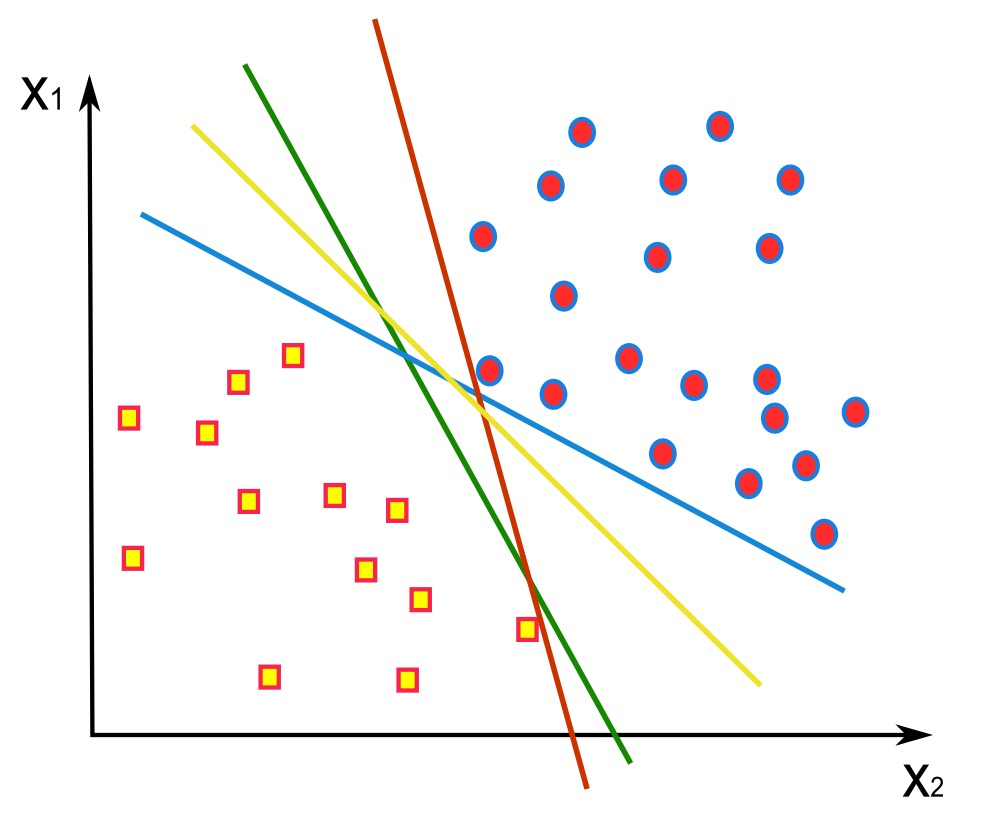
\includegraphics[width=1\textwidth]{2/figures/svm1.jpeg}
		\caption{Hiperplanos de separación(\cite{tecnica3})}
	\end{center}
\end{figure}

\begin{itemize}
\item \textbf{Margen Geométrico:}
\begin{itemize}
	\item El margen geométrico se define como:
	\[
	\gamma = \frac{1}{\|w\|}
	\]
	\item El hiperplano de separación óptimo maximiza este margen, mejorando la capacidad de generalización del modelo.
\end{itemize}

\item \textbf{Optimización del Margen:}
\begin{itemize}
	\item La optimización del margen geométrico implica minimizar la norma del vector de pesos \( w \).
	\item Esto se resuelve mediante un problema de programación cuadrática para encontrar el hiperplano óptimo y dos hiperplanos paralelos (H1 y H2) que maximicen la distancia entre ellos sin que haya datos entre estos hiperplanos.
\end{itemize}

\item \textbf{Vectores de Soporte:}
\begin{itemize}
	\item Los puntos de datos más cercanos al hiperplano de separación, llamados vectores de soporte, definen este hiperplano. Los demás puntos no afectan la solución del SVM.
\end{itemize}

\item \textbf{Formulación Dual:}
\begin{itemize}
	\item Se utiliza la formulación dual mediante multiplicadores de Lagrange para simplificar el problema.
	\item Esto permite que los datos de entrenamiento aparezcan solo como productos punto entre vectores, lo cual es fundamental para generalizar el procedimiento a casos no lineales.
	\item La Lagrangiana es:
	\[
	L(w, b, \alpha) = \frac{1}{2} \|w\|^2 - \sum_{i=1}^{l} \alpha_i \left[ y_i \left( w \cdot x_i + b \right) - 1 \right]
	\]
\end{itemize}

\item \textbf{Solución Dual:}
\begin{itemize}
	\item La solución del problema dual implica derivar con respecto a \( w \) y \( b \) y luego sustituir estas derivadas en la Lagrangiana original:
	\[
	\frac{\partial L(w, b, \alpha)}{\partial w} = w - \sum_{i=1}^{l} \alpha_i y_i x_i = 0 \Rightarrow w = \sum_{i=1}^{l} \alpha_i y_i x_i
	\]
	\[        \frac{\partial L(w, b, \alpha)}{\partial b} = - \sum_{i=1}^{l} \alpha_i y_i = 0 \Rightarrow \sum_{i=1}^{l} \alpha_i y_i = 0        \]
	\item Los vectores de soporte son aquellos con \( \alpha_i > 0 \), y son cruciales para definir los hiperplanos \( H_1 \) y \( H_2 \).
\end{itemize}
\end{itemize}
 \begin{figure}[H]
	\begin{center}
		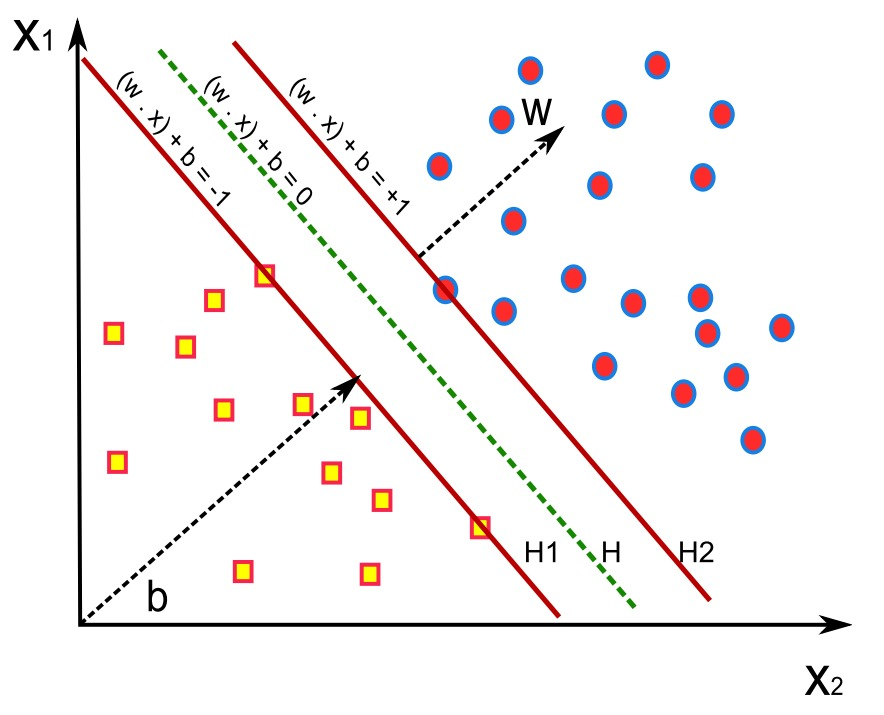
\includegraphics[width=0.8\textwidth]{2/figures/svm2.jpeg}
		\caption{Clasificador óptimo(\cite{tecnica3})}
	\end{center}
\end{figure}

\begin{itemize}
	\item El problema de aprendizaje presentado anteriormente es válido solo para datos linealmente separables, lo cual es raro en la vida real.
	\item En muchos casos, los datos de entrenamiento tienen intersecciones y no pueden ser separados linealmente sin errores.
	\item Los métodos de programación cuadrática anteriores no pueden ser usados en estos casos porque la condición $ y_i ( w \cdot x_i + b ) \geq 1 $ no puede ser satisfecha para todos los puntos de datos.
	\item En casos de intersección, algunos puntos de datos no pueden ser clasificados correctamente, y los valores correspondientes de $ \alpha_i $ tienden a infinito.
	\item Para manejar esto, se introduce el concepto de "soft margin", permitiendo una cierta cantidad de errores de clasificación.
	\item Se agregan variables de holgura no negativas $ \xi_i $ (slack variables) en la ecuación de separación:
	\[
	y_i ( w \cdot x_i + b ) \geq 1 - \xi_i \quad \text{con} \quad \xi_i \geq 0
	\]
\end{itemize}
 \begin{figure}[H]
	\begin{center}
		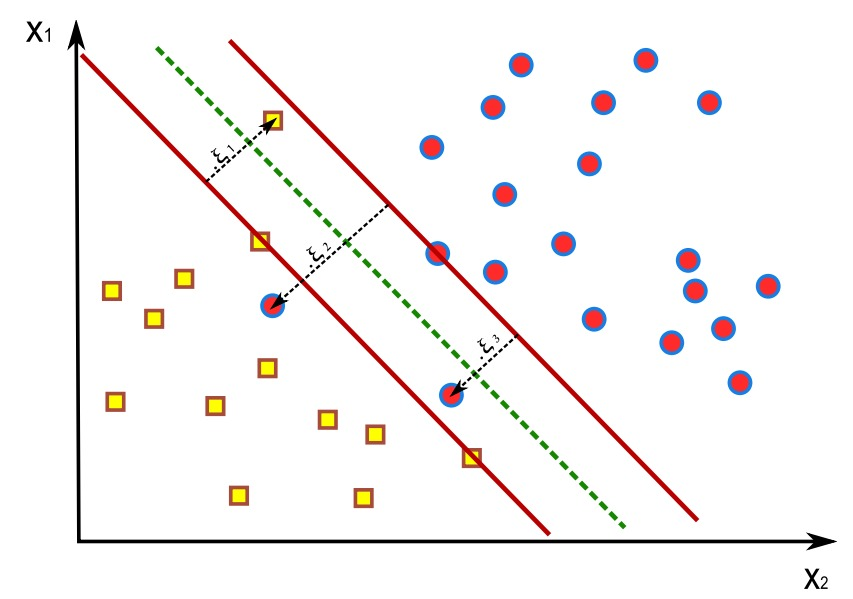
\includegraphics[width=0.8\textwidth]{2/figures/svm3.jpeg}
		\caption{Hiperplanos de margen suave.(\cite{tecnica3})}
	\end{center}
\end{figure}

 \begin{figure}[H]
	\begin{center}
		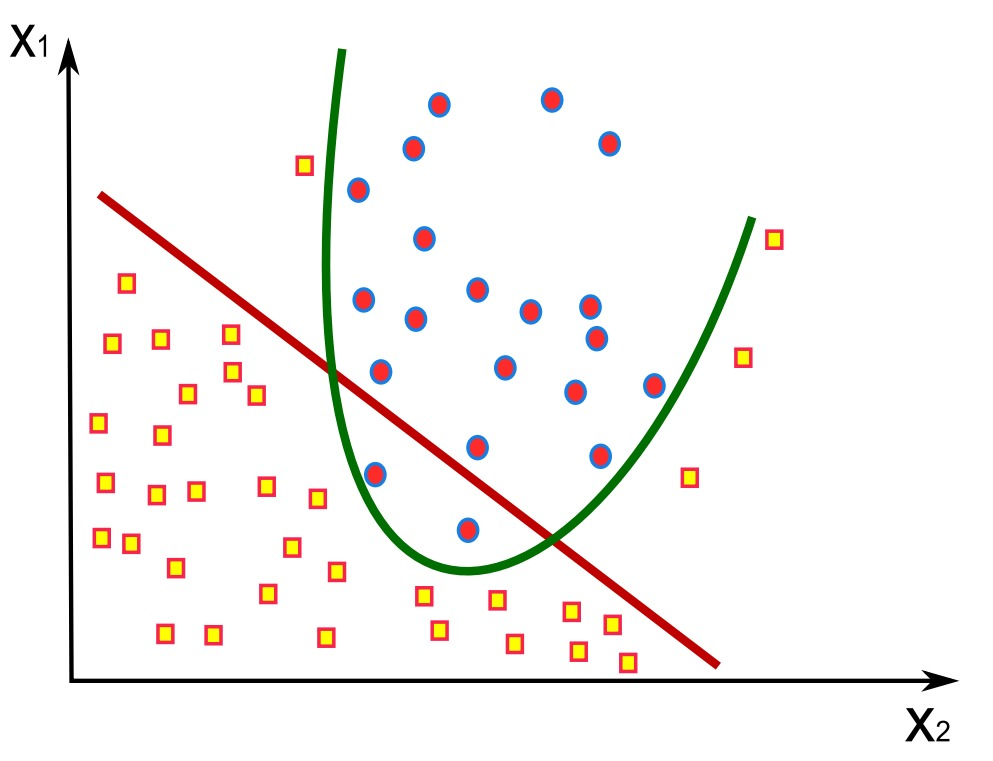
\includegraphics[width=0.8\textwidth]{2/figures/svm4.jpeg}
		\caption{Clasificacion no lineal.(\cite{tecnica3})}
	\end{center}
\end{figure}

En un SVM, el hiperplano óptimo se determina para maximizar la capacidad de generalización del modelo. Sin embargo, si la data de preparacion son linealmente unibles, el clasificador que se tuvo podria no tener una alta capacidad de generalización, incluso si los hiperplanos se determinan de manera óptima. Es decir, para engrandezer el hueco entre clases, el espacio de entrada original se transforma en un espacio de características altamente dimensional llamado ``espacio de características''.

La idea simple en la arquitectura de SVM no lineales es convertir los vectores que recben $x \in \mathbb{R}^n$ en vectores $U(x)$ de un cardumen de características altisimamente dimensional $F$ (donde $U$ representa la asignación: $\mathbb{R}^n \rightarrow \mathbb{R}^f$) y terminar la dificultad de clasificación lineal en este espacio de características. El conjunto de hipótesis consideradas será de la forma:

\[
f(x) = \sum_{i=1}^{l} w_i \phi_i(x) + b
\]

donde $\phi: X \rightarrow F$ es una asignación no lineal de un espacio de entrada a un espacio de características.

Una caracteristica de los componentes de aprendizaje lineales es que pueden expresarse en una vista dual, lo que significa que la ecuación anterior se puede expresar como una combinación lineal de los puntos de datos de entrenamiento. Por lo tanto, la regla de decisión puede evaluarse utilizando productos punto:

\[
f(x) = \sum_{i=1}^{l} \alpha_i y_i K(x_i, x) + b
\]

donde $K(x_i, x)$ es una función kernel que representa el producto punto en el espacio de características.

Los kernel son funciones que satisfacen ciertas propiedades y permiten calcular eficientemente la función de decisión. Algunos de los kernel más utilizados son:

\begin{itemize}
	\item Kernel lineal: $K(x_i, x_j) = (x_i \cdot x_j)$
	\item Kernel Gaussiano: $K(x_i, x_j) = e^{-\frac{||x_i - x_j||^2}{2\sigma^2}}$
	\item Kernel RBF: $K(x_i, x_j) = e^{-c||x_i - x_j||^2}$
	\item Kernel sigmoide: $K(x_i, x_j) = \tanh(g(x_i \cdot x_j) + m)$
\end{itemize}

La elección del kernel depende de las características de los datos y es necesario determinar los parámetros óptimos del kernel utilizado para obtener buenos resultados.

\subsubsection{Debilidades de SVM}
A pesar de la capacidad de generalización y las muchas ventajas de SVM, tienen algunas debilidades muy marcadas, entre las que se encuentran: la selección de parámetros, la complejidad algorítmica que afecta el tiempo de entrenamiento del clasificador en conjuntos de datos grandes, el desarrollo de clasificadores óptimos para problemas multiclase y el rendimiento de SVM en conjuntos de datos desequilibrados.

\paragraph{Complejidad algorítmica}

Limitación principal: alto costo computacional en conjuntos de datos voluminosos. Las SVM, si bien son herramientas poderosas, presentan una desventaja significativa: su elevado costo computacional al trabajar con conjuntos de datos de gran tamaño. La razón de esto reside en el crecimiento cuadrático de la matriz del kernel de entrenamiento con respecto al tamaño del conjunto de datos. Esta dependencia cuadrática deriva en un proceso de entrenamiento sumamente lento para conjuntos de datos voluminosos.

Los métodos de entrenamiento para SVM se pueden categorizar en selección de datos, descomposición, implementaciones geométricas, implementaciones paralelas y heurísticas. Sus ideas centrales y los algoritmos más representativos se presentan en esta sección.

\textbf{Métodos de selección de datos para SVM:} intentan disminuir el tamaño de los conjuntos de datos eliminando las instancias que no contribuyen a la definición del hiperplano separador óptimo. Estos métodos se basan en las instancias que están más cerca del límite de separación y se denominan vectores de soporte (SVs).

\textbf{Métodos de descomposición:} se basan en que el tiempo de entrenamiento se puede reducir si solo se tienen en cuenta las restricciones activas del problema QP. Un método similar a los métodos de conjunto activo para la optimización se aplica en estos métodos de descomposición.

\textbf{Métodos de implementación paralela:} dividen el conjunto de entrenamiento en subconjuntos independientes para entrenar SVM en diferentes procesadores.

\textbf{Métodos geométricos:} están basados en que calcular el hiperplano separador óptimo es equivalente a encontrar el par de puntos más cercanos que pertenecen a envolventes convexas.

\textbf{Métodos heurísticos:} incluyen técnicas como la inicialización de valores de parámetros para el inicio del problema QP, entre otros.



\subsubsection{Implementaciones de SVM}
\paragraph{Resumen de Implementaciones SVM:}
\begin{itemize}
	\item Actualmente existen varias implementaciones de Máquinas de Vectores de Soporte (SVM) en la literatura.
	\item El tiempo computacional varía entre las implementaciones debido a diferentes heurísticas utilizadas para resolver el problema de programación cuadrática.
	\item En conjuntos de datos grandes, las SVM enfrentan tiempos de entrenamiento enormes debido a su complejidad computacional casi cúbica.
\end{itemize}

\paragraph*{Enfoques para Mejorar el Tiempo de Entrenamiento de SVM:}
\begin{itemize}
	\item \textbf{Reducción de Datos:} Se centra en entrenar SVM con un subconjunto de datos probablemente vectores de soporte.
	\item \textbf{Fragmentación (Chunking):} Divide el problema en fragmentos más pequeños, resolviendo cada uno de forma iterativa.
	\item \textbf{Descomposición:} Resuelve una secuencia de problemas de optimización más pequeños para reducir la complejidad.
	\item \textbf{Optimización Secuencial Mínima (SMO):} Optimiza un subconjunto mínimo de dos puntos en cada iteración, escalando bien con conjuntos de datos grandes.
	\item \textbf{Reducción (Shrinking):} Acelera la optimización al reducir el número de valores del kernel necesarios.
	\item \textbf{Selección de Trabajo (Working Selection):} Selecciona un conjunto inicial de variables para optimizar SMO de manera eficiente.
\end{itemize}

\paragraph*{Beneficios de las Implementaciones SVM:}
\begin{enumerate}
	\item Pueden manejar conjuntos de datos grandes de manera eficiente.
	\item Soportan funciones de kernel estándar y personalizadas.
	\item Eficientes para clasificación multiclase y validación cruzada.
	\item Pueden manejar SVM ponderadas para datos desbalanceados.
	\item Proporcionan estimaciones de probabilidad.
\end{enumerate}

\paragraph*{Implementaciones SVM Populares:}
\begin{itemize}
	\item \textbf{SVMLight:} Utiliza técnicas de Selección de Trabajo y Reducción, eficiente para conjuntos de datos grandes.
	\item \textbf{SVMTorch:} Utiliza Selección de Trabajo y Reducción para problemas de regresión a gran escala.
	\item \textbf{Pegasos:} Implementa métodos de descomposición para reducción del tiempo de entrenamiento, adecuado para SVM no lineales.
	\item \textbf{LIBSVM:} Basado en SMO con algoritmo avanzado de selección de conjunto de trabajo, eficiente para conjuntos de datos grandes.
	\item \textbf{SVM Incremental:} Marco para aprendizaje incremental y adaptación de clasificadores SVM.
\end{itemize}

\begin{table}[H]
	\centering
	\caption{Implementaciones SVM}
	\label{tab:svm-implementations}
	\begin{tabular}{p{3cm}p{5cm}p{7cm}}
		\toprule
		\textbf{Implementación} & \textbf{Desarrollador} & \textbf{Código Fuente y Universidad} \\
		\midrule
		SVMTorch & Ronan Collobert and Samy Bengio & C++ - Université de Montréal \\
		Pegasos & Shai Shalev-Shwartz & C++ - The Hebrew University of Jerusalem\\
		LibSVM & Chih-Chung Chang and Chih-Jen Lin & C and Java - National Taiwan University \\
		SVMLight & Thorsten Joachims & C - Cornell University \\
		Incremental SVM & Chris Diehl & M - Carnegie Mellon \\
		\bottomrule
	\end{tabular}
\end{table}

\subsubsection{Aplicaciones en problemas del mundo real en Clasificacion de imagenes}
\paragraph{Clasificación de Cálculos Renales:} En \cite{svmm1}, se emplean filtros de mediana y Gaussiano, y se aplica un enmascaramiento no agudo para mejorar las imágenes. Se utilizan operaciones morfológicas y segmentación basada en entropía para encontrar la región de interés, y luego se emplean técnicas de clasificación KNN y SVM para el análisis de imágenes de cálculos renales.

\paragraph{Detección Temprana de Melanoma:} En \cite{svmm2}, se presenta un dispositivo de manejo con bajo costo y alto rendimiento para mejorar la detección temprana de melanoma en atención primaria. Se propone un sistema de hardware dinámico para implementar un clasificador SVM en cascada en FPGA para la detección temprana de melanoma.

\paragraph{Reconocimiento de Expresiones Faciales:} En \cite{svmm3}, se presenta un marco para el reconocimiento de expresiones independiente de la persona mediante el aprendizaje de múltiples tipos de características faciales a través del aprendizaje de múltiples núcleos en SVM multiclase.

\paragraph{Reconocimiento de Gestos de Mano:} Se aborda el reconocimiento de signos indios basado en técnicas de reconocimiento de gestos de mano dinámicos en escenarios en tiempo real. Se utilizan momentos de Hu y trayectorias de movimiento para la extracción de características y la clasificación de gestos mediante SVM.

\paragraph{Clasificación de Imágenes Hiperespectrales:} En \cite{svmm4}, se propone una técnica para la clasificación espectral-espacial de imágenes hiperespectrales que combina la clasificación pixel a pixel con SVM y la información contextual espacial con un enfoque de Campo Aleatorio de Markov para refinar los resultados de la clasificación.

\paragraph{Selección de Características para la Clasificación de Masas Mammográficas:} En \cite{svmm5}, se abordan métodos de selección de características para la clasificación de masas en mamografías, integrando un procedimiento basado en eliminación recursiva de características SVM con una selección de características de información mutua normalizada.

\paragraph{Clasificación de Imágenes mediante SVM con Kernel de Intersección de Histogramas:} En \cite{svmm6}, se propone un método para la clasificación de imágenes mediante SVM con kernel de intersección de histogramas. Se presenta un solver de kernel de intersección de histogramas determinista y escalable.

\paragraph{Decodificación de Códigos QR a Color:} En \cite{svmm7}, se proponen dos enfoques para resolver problemas de decodificación de códigos QR a color. LSVM-CMI y QDA-CMI, que modelan conjuntamente diferentes tipos de distorsión cromática.


\begin{figure}[H]
\begin{center}
	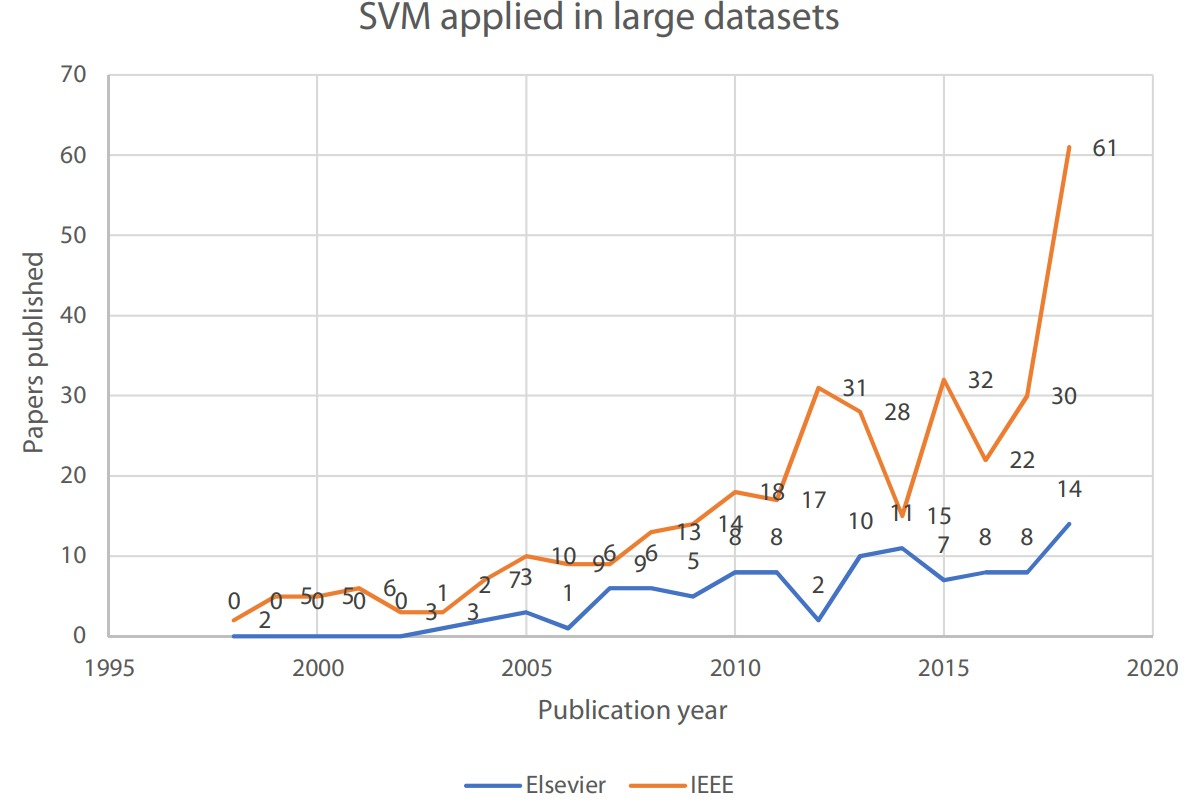
\includegraphics[width=1\textwidth]{2/figures/svm5.jpeg}
	\caption{Número de publicaciones, en capítulos de libros y revistas, por año que contienen los términos de búsqueda SVM y Grandes conjuntos de datos.(\cite{tecnica3})}
\end{center}
\end{figure}

\begin{figure}[H]
\begin{center}
	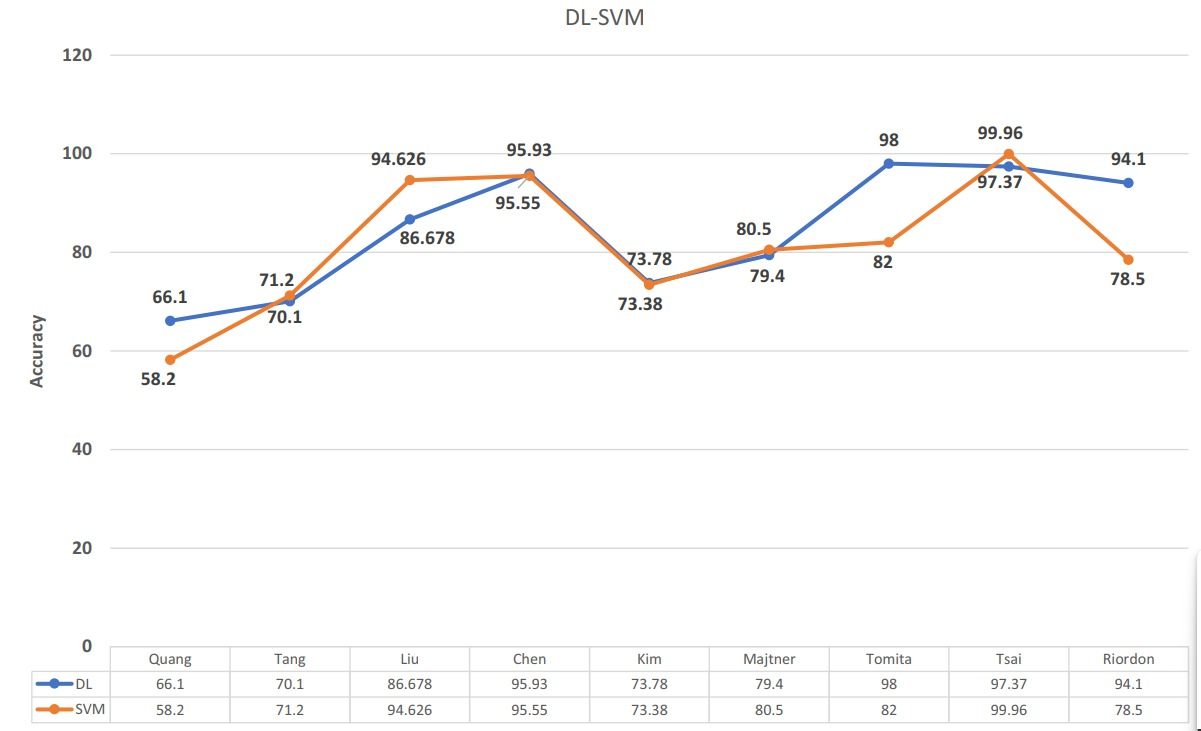
\includegraphics[width=1\textwidth]{2/figures/svm6.jpeg}
	\caption{Rendimiento de SVM frente a Aprendizaje profundo(\cite{tecnica3})}
\end{center}
\end{figure}

\subsubsection{Conclusiones}
Debido a sus sólidos fundamentos teóricos y capacidad de generalización, entre otras ventajas, las SVM han sido implementadas en muchas aplicaciones del mundo real. Los algoritmos SVM han sido implementados en diversos campos de investigación como: categorización de texto (e hipertexto), detección de pliegues de proteínas y homología remota, clasificación de imágenes, bioinformática (clasificación de proteínas y cáncer), reconocimiento de caracteres escritos a mano, detección de rostros, control predictivo generalizado y muchos más. Muchos investigadores han demostrado que las SVM son mejores que otras técnicas de clasificación actuales. Sin embargo, a pesar de que las SVM tienen algunas limitaciones relacionadas con la selección de parámetros, la complejidad algorítmica, conjuntos de datos multiclase y conjuntos de datos desequilibrados, han sido implementadas en muchos problemas de clasificación de la vida real debido a sus buenos fundamentos teóricos y rendimiento de generalización.

Es importante mencionar que las SVM no son tan populares cuando los conjuntos de datos son muy grandes porque algunas implementaciones de SVM requieren un tiempo de entrenamiento enorme o, en otros casos, cuando los conjuntos de datos están desequilibrados, la precisión de las SVM es pobre. Hemos presentado algunas técnicas para enfrentar estos desequilibrios en los conjuntos de datos. Este artículo describe detalladamente las principales desventajas de las SVM y muchos algoritmos implementados para enfrentar estas desventajas, y cita los trabajos de investigadores que han enfrentado estas desventajas
 \subsection{Redes neuronales convolucionales: Review of Image Classification Algorithms Based on Convolutional Neural Networks \citep*{tecnica2}}
 Este artículo destaca el papel crucial de las redes neuronales convolucionales (CNN) en la clasificación de imágenes desde 2012. Explora su evolución desde modelos básicos hasta arquitecturas avanzadas y su influencia en áreas de reconocimiento visual. Compara métodos de clasificación y analiza el impacto de CNN en diversas aplicaciones, subrayando tendencias actuales en el campo. La introducción aborda la importancia de la clasificación de imágenes y su evolución desde la extracción manual de características hasta el uso de CNN, inspiradas en la biología. Modelos como LeNet-5, AlexNet y ZFNet han mejorado significativamente el rendimiento en este ámbito.
 
 A pesar de que las CNN se diseñaron originalmente para la visión por computadora, su aplicación exitosa en el análisis de imágenes de teledetección ha llevado a la necesidad de un análisis sistemático de los métodos de clasificación de imágenes basados en CNN. Este artículo se dedica a detallar el desarrollo de casi todas las arquitecturas de CNN típicas en tareas de clasificación de imágenes, con el objetivo de proporcionar inspiración para el diseño de modelos CNN en el campo del análisis de imágenes de teledetección.
 
 
 \subsubsection{Visión general de las CNN}
 La CNN tiene una estructura principal compuesta por capas convolucionales, de agrupación, de activación no lineal y completamente conectadas. Después de preprocesar la imagen, se introduce en la red a través de la capa de entrada, se procesa mediante capas convolucionales y de agrupación alternadas, y finalmente se clasifica mediante la capa completamente conectada. En comparación con MLP, la CNN agrega capas convolucionales y de agrupación, lo que mejora el rendimiento en términos de tamaño del modelo y capacidad de procesamiento. La capa convolucional identifica eficazmente la correlación entre las características de los píxeles de la imagen, mientras que la capa de agrupación reduce la carga computacional y la sensibilidad excesiva a la posición. La CNN asegura cierto grado de invarianza ante cambios en la imagen como desplazamientos, escalados y distorsiones.
 
 Para CNNs con una cierta profundidad, la operación de convolución de múltiples capas convolucionales puede extraer diferentes características de la entrada. La capa convolucional inferior generalmente extrae características comunes como textura, líneas y bordes, mientras que la capa superior extrae características más abstractas. La capa convolucional tiene varios núcleos de convolución con parámetros aprendibles, que son matrices compuestas por pesos aprendibles. Estas matrices de pesos suelen ser de tamaño 3 × 3, 5 × 5 y 7 × 7, con una longitud y ancho iguales y un número impar. Normalmente, la capa convolucional ingresará a los mapas de características. La matriz de pesos del núcleo de convolución corresponde al área local del mapa de características de conexión, y el núcleo de convolución realiza operaciones de convolución secuenciales en el área del mapa de características mediante deslizamiento. 
 
 La fórmula para la salida de una superficie de características en la capa convolucional puede expresarse aproximadamente como:
 
 \[ \text{{feature\_surface\_out}} = \sum_{i=1}^{N} M_i * W_i + B \]
 
 Donde \( M_i \) representa una superficie de características de los mapas de características de entrada, \( W_i \) es la matriz de pesos del núcleo de convolución, la matriz de sesgo es \( B \), \( f(\cdot) \) es la función de activación no lineal y \( \text{{feature\_surface\_out}} \) es una superficie de características de salida.
 

 \begin{figure}[H]
 	\begin{center}
 		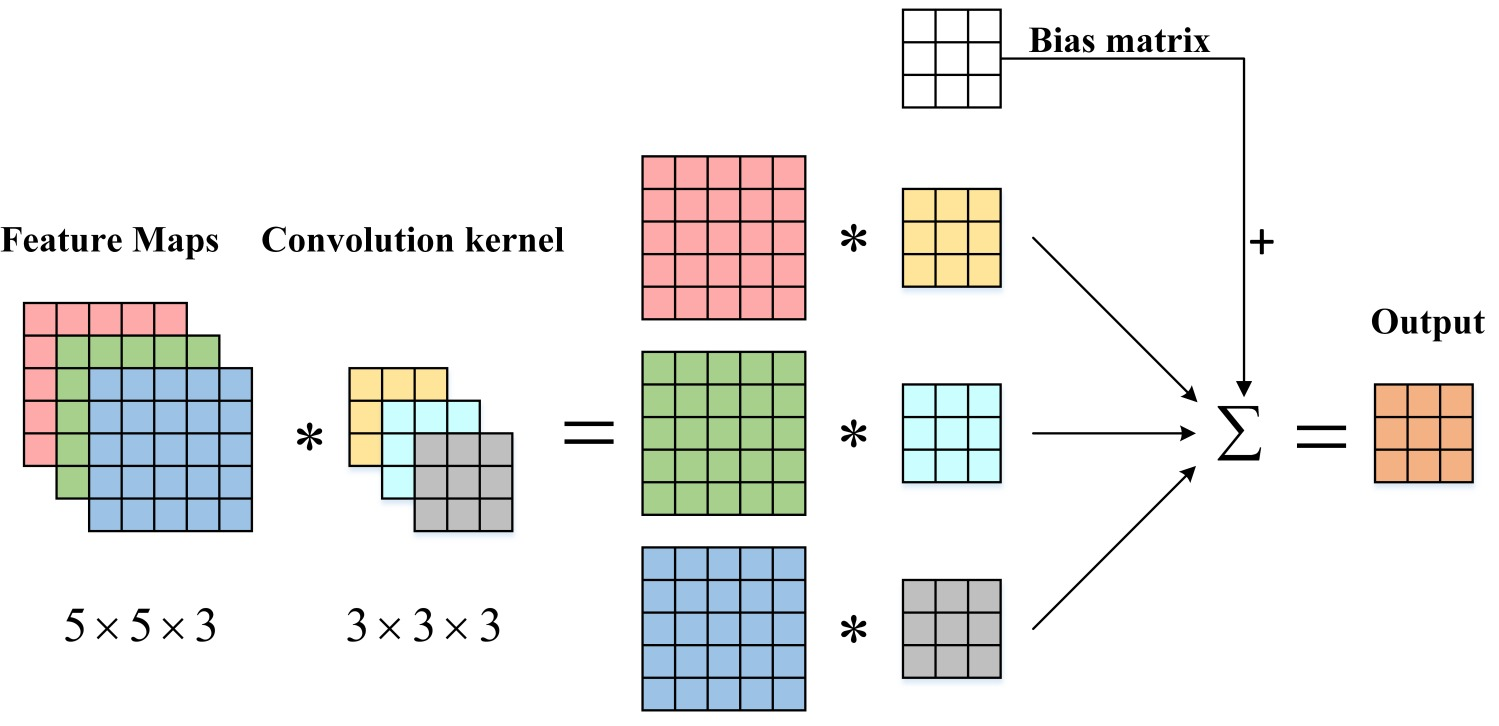
\includegraphics[width=1\textwidth]{2/figures/cnn1.jpeg}
 		\caption{Diagrama esquemático del proceso de convolución(\cite{tecnica2})}
 	\end{center}
 \end{figure}
 
 La capa de agrupación generalmente sigue a la capa convolucional. Las principales razones para usar la capa de agrupación son: realizar un procesamiento de submuestreo y reducción de dimensionalidad en la imagen de entrada para reducir el número de conexiones de la capa convolucional, reduciendo así la carga computacional de la red; lograr invariancia de escala, invariancia de traslación e invariancia de rotación de la imagen de entrada; hacer que el mapa de características de salida sea más robusto ante la distorsión y el error de una sola neurona.
 
 Los métodos de agrupación más utilizados son el promedio y el máximo. Aunque existen otras formas de agrupación que pueden mitigar de manera más efectiva el sobreajuste de las redes neuronales convolucionales, como la Agrupación Lp, Agrupación Mixta, Agrupación Estocástica, Agrupación de Pirámide Espacial (SPP) y Agrupación Ordenada Multiescala, entre otros. Sin embargo, para el modelo clásico de red neuronal convolucional, aunque la mejor operación de agrupación no es la agrupación promedio o la agrupación máxima, son los dos métodos más clásicos. En [72], Bourbeau realizó principalmente un análisis teórico sobre el rendimiento de la agrupación promedio y la agrupación máxima. La operación de agrupación satisface la siguiente relación general entre el tamaño de las matrices de entrada y salida:
 
\[o = \left( \frac{{i - k}}{s} \right) + 1 \]

 \begin{figure}[H]
	\begin{center}
		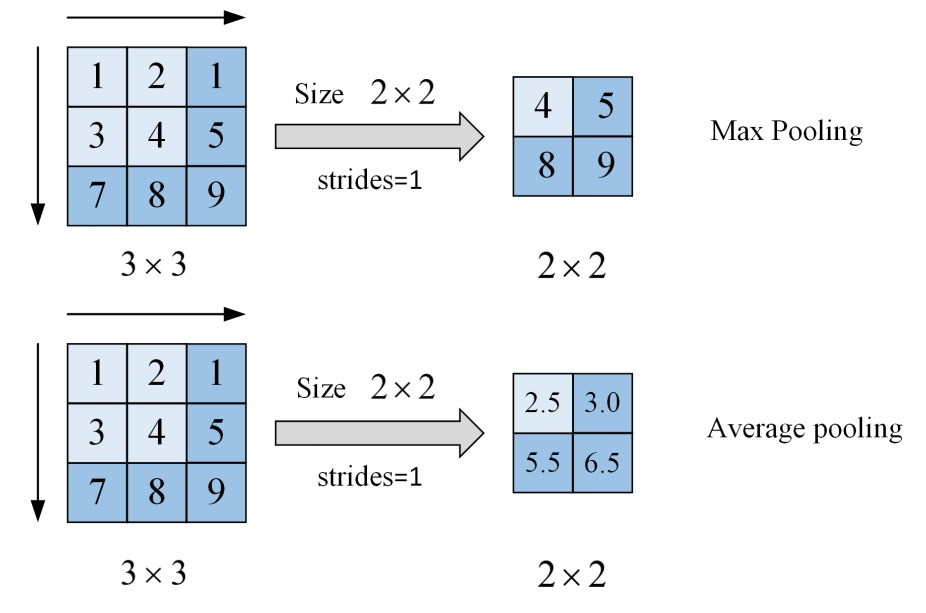
\includegraphics[width=1\textwidth]{2/figures/cnn2.jpeg}
		\caption{Agrupación máxima y agrupación promedio, no implica relleno cero.(\cite{tecnica2})}
	\end{center}
\end{figure}
 
 El propósito de la función de activación es establecer una relación funcional entre la entrada y la salida, introduciendo así un componente no lineal en la red neural. Una función de activación adecuada puede mejorar significativamente el rendimiento de la red. Algunas funciones comunes incluyen sigmoides y Tanh, que son no linealidades saturantes. Sin embargo, para abordar los problemas asociados con estas no linealidades saturantes, se han propuesto funciones no saturantes como ReLU, Leaky ReLU, PReLU, RReLU y ELU. Estas funciones no saturantes son mucho más rápidas para el entrenamiento por descenso de gradiente, lo que resulta en redes mucho más eficientes. Las neuronas con funciones no saturantes se conocen como Unidades Lineales Rectificadas (ReLUs).
 
 En la arquitectura de las CNN, la clasificación final se logra desde la capa de salida, generalmente la última capa de la capa completamente conectada (FC layer). Las diferentes funciones de pérdida también afectan el rendimiento de la arquitectura de la CNN y se aplican a diferentes tareas visuales (como la clasificación de imágenes, reconocimiento facial y reconocimiento de objetos). La función de pérdida más comúnmente utilizada es Softmax+Entropía Cruzada, con muchas versiones mejoradas basadas en ella, como center-loss, L-Softmax, A-Softmax, AM-Softmax, PEDCC-loss, entre otras, que desempeñan un papel importante en diferentes tareas visuales.
 
\begin{table}[H]
	\centering
	\caption{Funciones de pérdida comunes para modelos CNN.}
	\label{tab:loss_functions}
	\begin{tabular}{p{3cm}p{5cm}p{7cm}}
		\toprule
		Función de Pérdida & Ecuación & Característica \\
		\bottomrule
		L1 (MAE) & $\text{Pérdida}(y, y^*) = \frac{1}{m} \sum_{i=1}^{m} |y^*_i - y_i|$ & Ampliamente utilizado en problemas de regresión. La pérdida L1 se denomina error absoluto medio (MAE). \\
		\midrule
		L2 (MSE) & $\text{Pérdida}(y, y^*) = \frac{1}{m} \sum_{i=1}^{m} (y^*_i - y_i)^2$ & Ampliamente utilizado en problemas de regresión. La pérdida L2 se denomina error cuadrático medio (MSE). \\
		\midrule
		Softmax + Entropía Cruzada & $\text{Pérdida}(y, y^*) = - \sum_{i} y_i \log\left(\frac{\sum_{m}^{i=1} y_i}{\sum_{i}^{m} y_i}\right)$ & Esta función suele emplearse como sustitución del MSE en problemas de clasificación multi-clase. También se utiliza comúnmente en modelos CNN. \\
		\midrule
	\end{tabular}
\end{table}


El flujo de datos en la arquitectura CNN se introduce básicamente en la sección anterior. Entendemos claramente que el entrenamiento de la red se basa en el paso fundamental de la actualización del gradiente, es decir, necesita calcular el gradiente de la función objetivo (función de pérdida) aplicando una derivada de primer orden con respecto a los parámetros de la red, y luego la información del gradiente se transfiere a la capa de red anterior en forma de cálculo de derivada parcial para lograr la actualización de los parámetros de aprendizaje de cada capa de red. La función del optimizador es proporcionar una manera de hacer que la actualización del gradiente sea más razonable, es decir, la macroscópica es que toda la red puede converger más rápido, un valor óptimo local más pequeño (pérdida más pequeña), cálculos más baratos, etc.

\begin{table}[H]
	\centering
	\caption{Métodos de optimización para modelos CNN.}
	\label{tab:optimization_methods}
	\begin{tabular}{p{2.5cm}p{5cm}p{7cm}}
		\toprule
		Nombre & Método & Características \\
		\midrule
		Batch Gradient Descent (BGD) & Calcula el gradiente de todo el conjunto de entrenamiento y posteriormente utiliza este gradiente para actualizar los parámetros. & 1. Para un conjunto de datos de pequeño tamaño, el modelo CNN converge más rápido y crea un gradiente extra estable utilizando BGD. 2. Generalmente no es adecuado para un conjunto de entrenamiento grande. 3. Requiere una cantidad sustancial de recursos. \\
		\midrule
		Stochastic Gradient Descent (SGD) & Muestrea seleccionando arbitrariamente parte del conjunto de entrenamiento. & 1. Para un conjunto de entrenamiento de gran tamaño, esta técnica es más eficiente en memoria y mucho más rápida que BGD. 2. Se introduce aleatoriedad y ruido debido a sus actualizaciones frecuentes. Su convergencia no es estable, pero la expectativa sigue siendo igual al descenso de gradiente correcto. \\
		\midrule
		Mini-batch Gradient Descent & Divide las muestras de entrenamiento en varios mini lotes, y luego se realiza la actualización de parámetros siguiendo el cálculo del gradiente en cada mini lote. & Este método combina las ventajas técnicas de SGD y SGD, que tienen una convergencia estable, más eficiencia computacional y una eficacia de memoria extra. \\
		\midrule
		Momentum & Introduce un parámetro de momento en SGD que acumula información de gradiente histórica. & Cuando el entrenamiento cae en un mínimo local, la información del gradiente con momento puede ayudar a la red a escapar y encontrar el mínimo global. \\
		\midrule
		Adaptive Moment Estimation (Adam) & Calcula una tasa de aprendizaje adaptativa para cada parámetro en el modelo. & Se combinan las ventajas del momento y RMSprop. Es ampliamente utilizado en el aprendizaje profundo y representa la última tendencia de optimización. \\
		\bottomrule
	\end{tabular}
\end{table}
 \subsubsection{Clasificación de imágenes basada en CNN}
 En general, la clasificación de imágenes implica extraer características de la imagen manualmente o mediante métodos de aprendizaje de características, y luego usar un clasificador para identificar la categoría del objeto. Antes del aprendizaje profundo, se utilizaba ampliamente el modelo de Bag of Words, que involucraba tres procesos: extracción de características de bajo nivel, codificación de características y diseño de clasificador. Este método tradicional fue común hasta 2012, siendo utilizado en competiciones como PASCAL VOC y ILSVRC 2010. Sin embargo, la aparición de las CNNs revolucionó la clasificación de imágenes, permitiendo un aprendizaje de características más eficaz y un proceso de clasificación de extremo a extremo que no requiere la extracción manual de características, superando las limitaciones de los métodos tradicionales. Esta sección presenta los modelos clásicos de clasificación de imágenes basados en CNN a lo largo del tiempo.
 
 

 \begin{itemize}
 	\item \textbf{LeNet Network:} En 1998, Lecun  desarrolló el modelo LeNet-5 para clasificar imágenes digitalmente, superando a otros métodos de la época y utilizando retropropagación por primera vez en CNNs. LeNet-5, con 7 capas y ~60k parámetros, se divide en un área de convolución y un área FC, utilizando la función de activación sigmoid y el clasificador softmax. Aunque tuvo buenos resultados en MNIST, su rendimiento en conjuntos de datos más grandes fue limitado debido a la complejidad computacional y la falta de investigación en inicialización de parámetros y algoritmos de optimización. Eventualmente, fue superado por otros métodos de aprendizaje automático como SVM.
 	\item \textbf{AlexNet Network:} En 2012, AlexNet, desarrollado por Krizhevsky et al., ganó la ILSVR 2012 con gran ventaja, demostrando que las características aprendidas superan a las diseñadas manualmente. Utilizó procesamiento paralelo entre GPUs debido a las limitaciones de la GPU GTX 580. AlexNet tiene 8 capas y ~60M parámetros, con 5 capas de convolución y 3 capas FC. Requiere un tamaño de convolución mayor para las imágenes más grandes de ImageNet. Mejoras clave incluyen:
 	ReLU: Aceleró la convergencia y redujo la desaparición del gradiente.
 	Dropout: Controló la complejidad del modelo y mitigó el sobreajuste.
 	Aumento de datos: Usó técnicas como volteo, recorte y cambios de color para ampliar conjuntos de datos y reducir el sobreajuste.
 	Pooling superpuesto: Mejoró la precisión del modelo y alivió el sobreajuste.
 	

  
   \begin{figure}[H]
  	\begin{center}
  		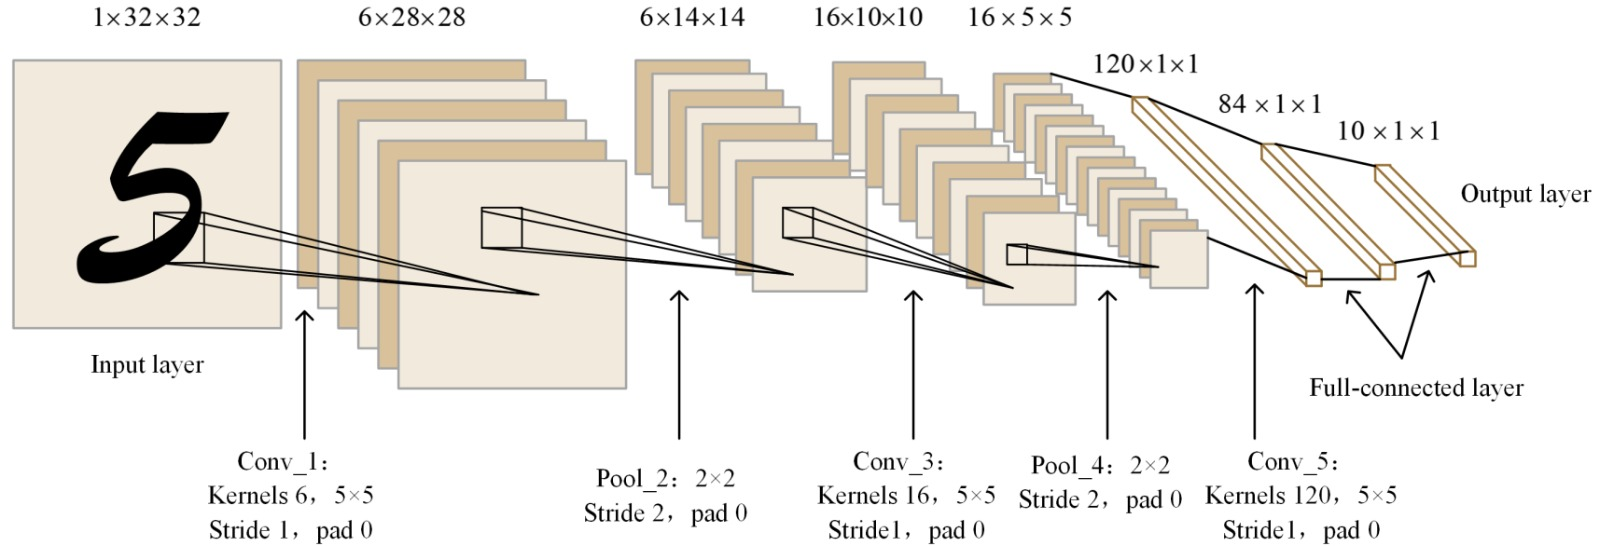
\includegraphics[width=1\textwidth]{2/figures/cnn3.jpeg}
  		\caption{La arquitectura de la red LeNet-5. La forma de salida es canal × altura × anchura. Cada capa convolucional
  			Utiliza tallas 5 × 5, relleno 0, zancadas 1. Cada capa de agrupación tiene un tamaño de 2 × 2 y zancadas 2.(\cite{tecnica2})}
  	\end{center}
  \end{figure}
  	\item \textbf{VGGNet:} En 2014, Simonyan et al. propusieron el modelo VGG, obteniendo el segundo lugar en ILSVR 2014. Similar a AlexNet, VGG usa una estructura de área de convolución seguida de área FC. Utiliza varias capas de convolución idénticas seguidas de una capa de pooling que reduce la altura y anchura a la mitad. VGG-16, una variante con 16 capas, conecta cinco bloques en serie y termina con dos capas FC de 4096 neuronas y una capa de salida de 1000 clasificaciones.
  	
  	Mejoras respecto a AlexNet:
  	
  	Red modular: Uso de módulos básicos para construir el modelo.
  	Convoluciones más pequeñas: Filtros de 3x3 que aumentan la profundidad y reducen parámetros comparado con filtros más grandes.
  	Entrenamiento multi-escala: Escala la imagen de entrada y la recorta aleatoriamente, logrando aumento de datos y previniendo el sobreajuste.
  
     \begin{figure}[H]
  	\begin{center}
  		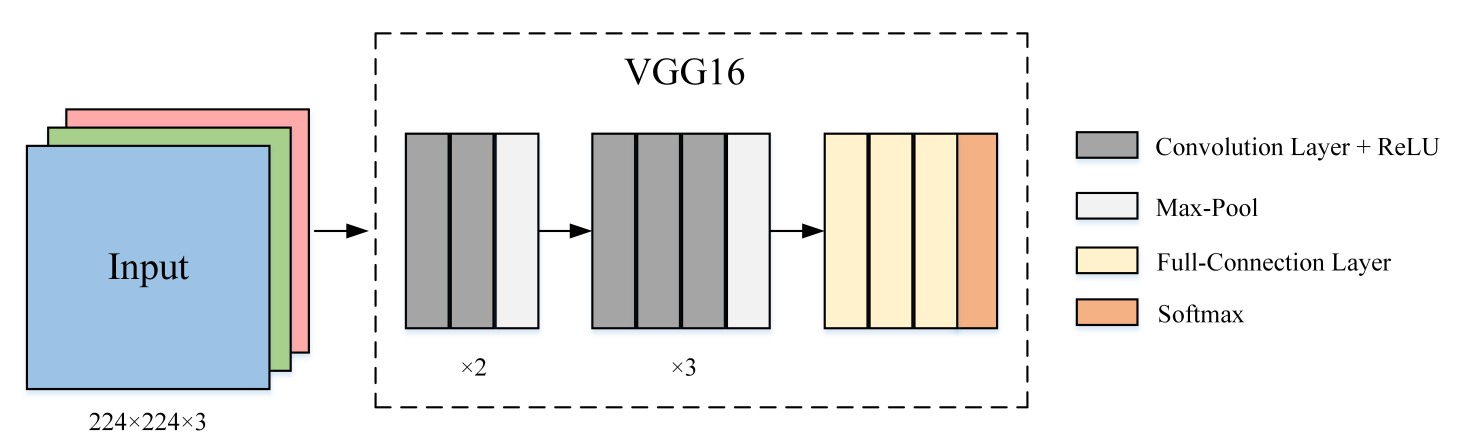
\includegraphics[width=1\textwidth]{2/figures/cnn4.jpeg}
  		\caption{ La arquitectura de la red VGG-16. Conv: tamaño = 3 × 3, zancada = 1, relleno = 1. Piscina:
  			tamaño = 3 × 3, zancada = 2.
  			(\cite{tecnica2})}
  	\end{center}
  \end{figure}
  \item \textbf{ GoogLeNet/InceptionV1 to V4:}En 2014, GoogLeNet, propuesta por Christian Szegedy et al., ganó el campeonato de ILSVR 2014 introduciendo el módulo Inception.
  
  InceptionV1:
  
  Tiene 22 capas y alrededor de 6 millones de parámetros.
  El módulo Inception contiene 4 ramas paralelas: tres con capas de convolución de diferentes tamaños (1x1, 3x3, 5x5) y una con una capa de max-pooling, seguido de convolución 1x1.
  Mejora la adaptabilidad y la fusión multi-escala al aumentar el ancho del modelo.
  
  InceptionV2:
  
  Reemplaza convoluciones de 5x5 con dos convoluciones de 3x3 para reducir el tiempo de cálculo.
  Introduce Batch Normalization (BN) para estabilizar y acelerar el entrenamiento mediante la normalización de las entradas de las capas.
  
  InceptionV3:
  
  Utiliza convoluciones factoradas y asimétricas, reemplazando una convolución 3x3 por una 1x3 seguida de una 3x1 para reducir los parámetros y mejorar la eficiencia computacional.
  Implementa reducción del tamaño de la cuadrícula mediante operaciones de pooling y convoluciones con stride 2.
  Introduce técnicas adicionales para optimizar la eficiencia computacional y prevenir el sobreajuste, como el uso de múltiples tamaños de escala para las imágenes de entrada.
    \begin{figure}[H]
  	\begin{center}
  		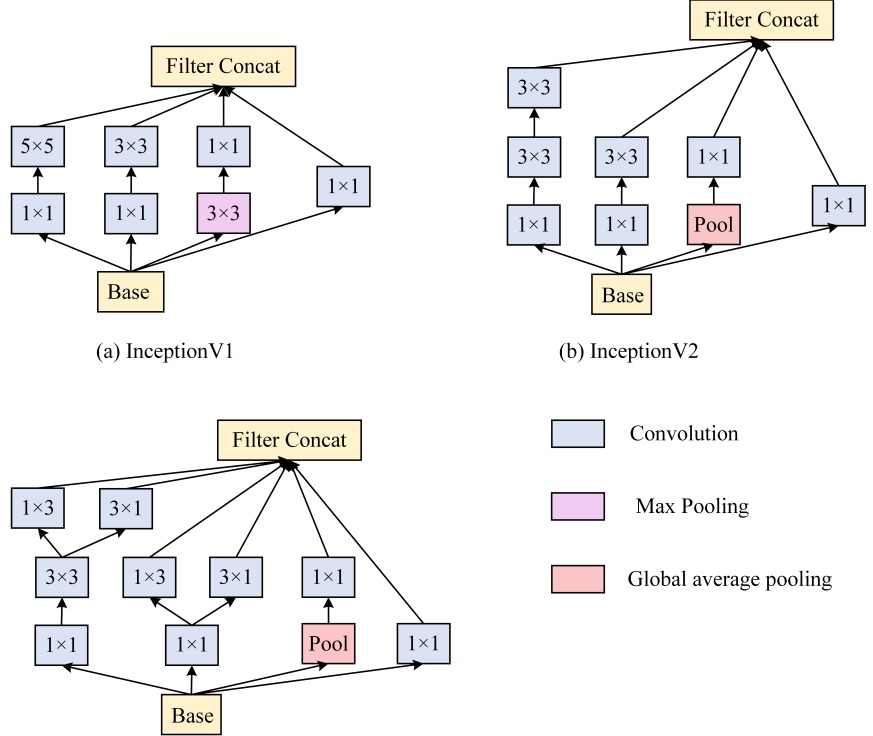
\includegraphics[width=1\textwidth]{2/figures/cn55.jpeg}
  		\caption{  Módulo InceptionV1 a V3
  			(\cite{tecnica2})}
  	\end{center}
  	\end{figure}
  InceptionV4:
  
  Reduce la complejidad de InceptionV3 mediante la unificación de las opciones de cada bloque de Inception.Los bloques de Inception y de Reducción son utilizados para simplificar y optimizar la arquitectura. El "stem" de la arquitectura se modifica para ser más uniforme y mejorar la eficiencia. Se optimiza el uso de memoria durante la retropropagación, permitiendo entrenar el modelo sin particionar réplicas.
  
   \begin{figure}[H]
  	\begin{center}
  		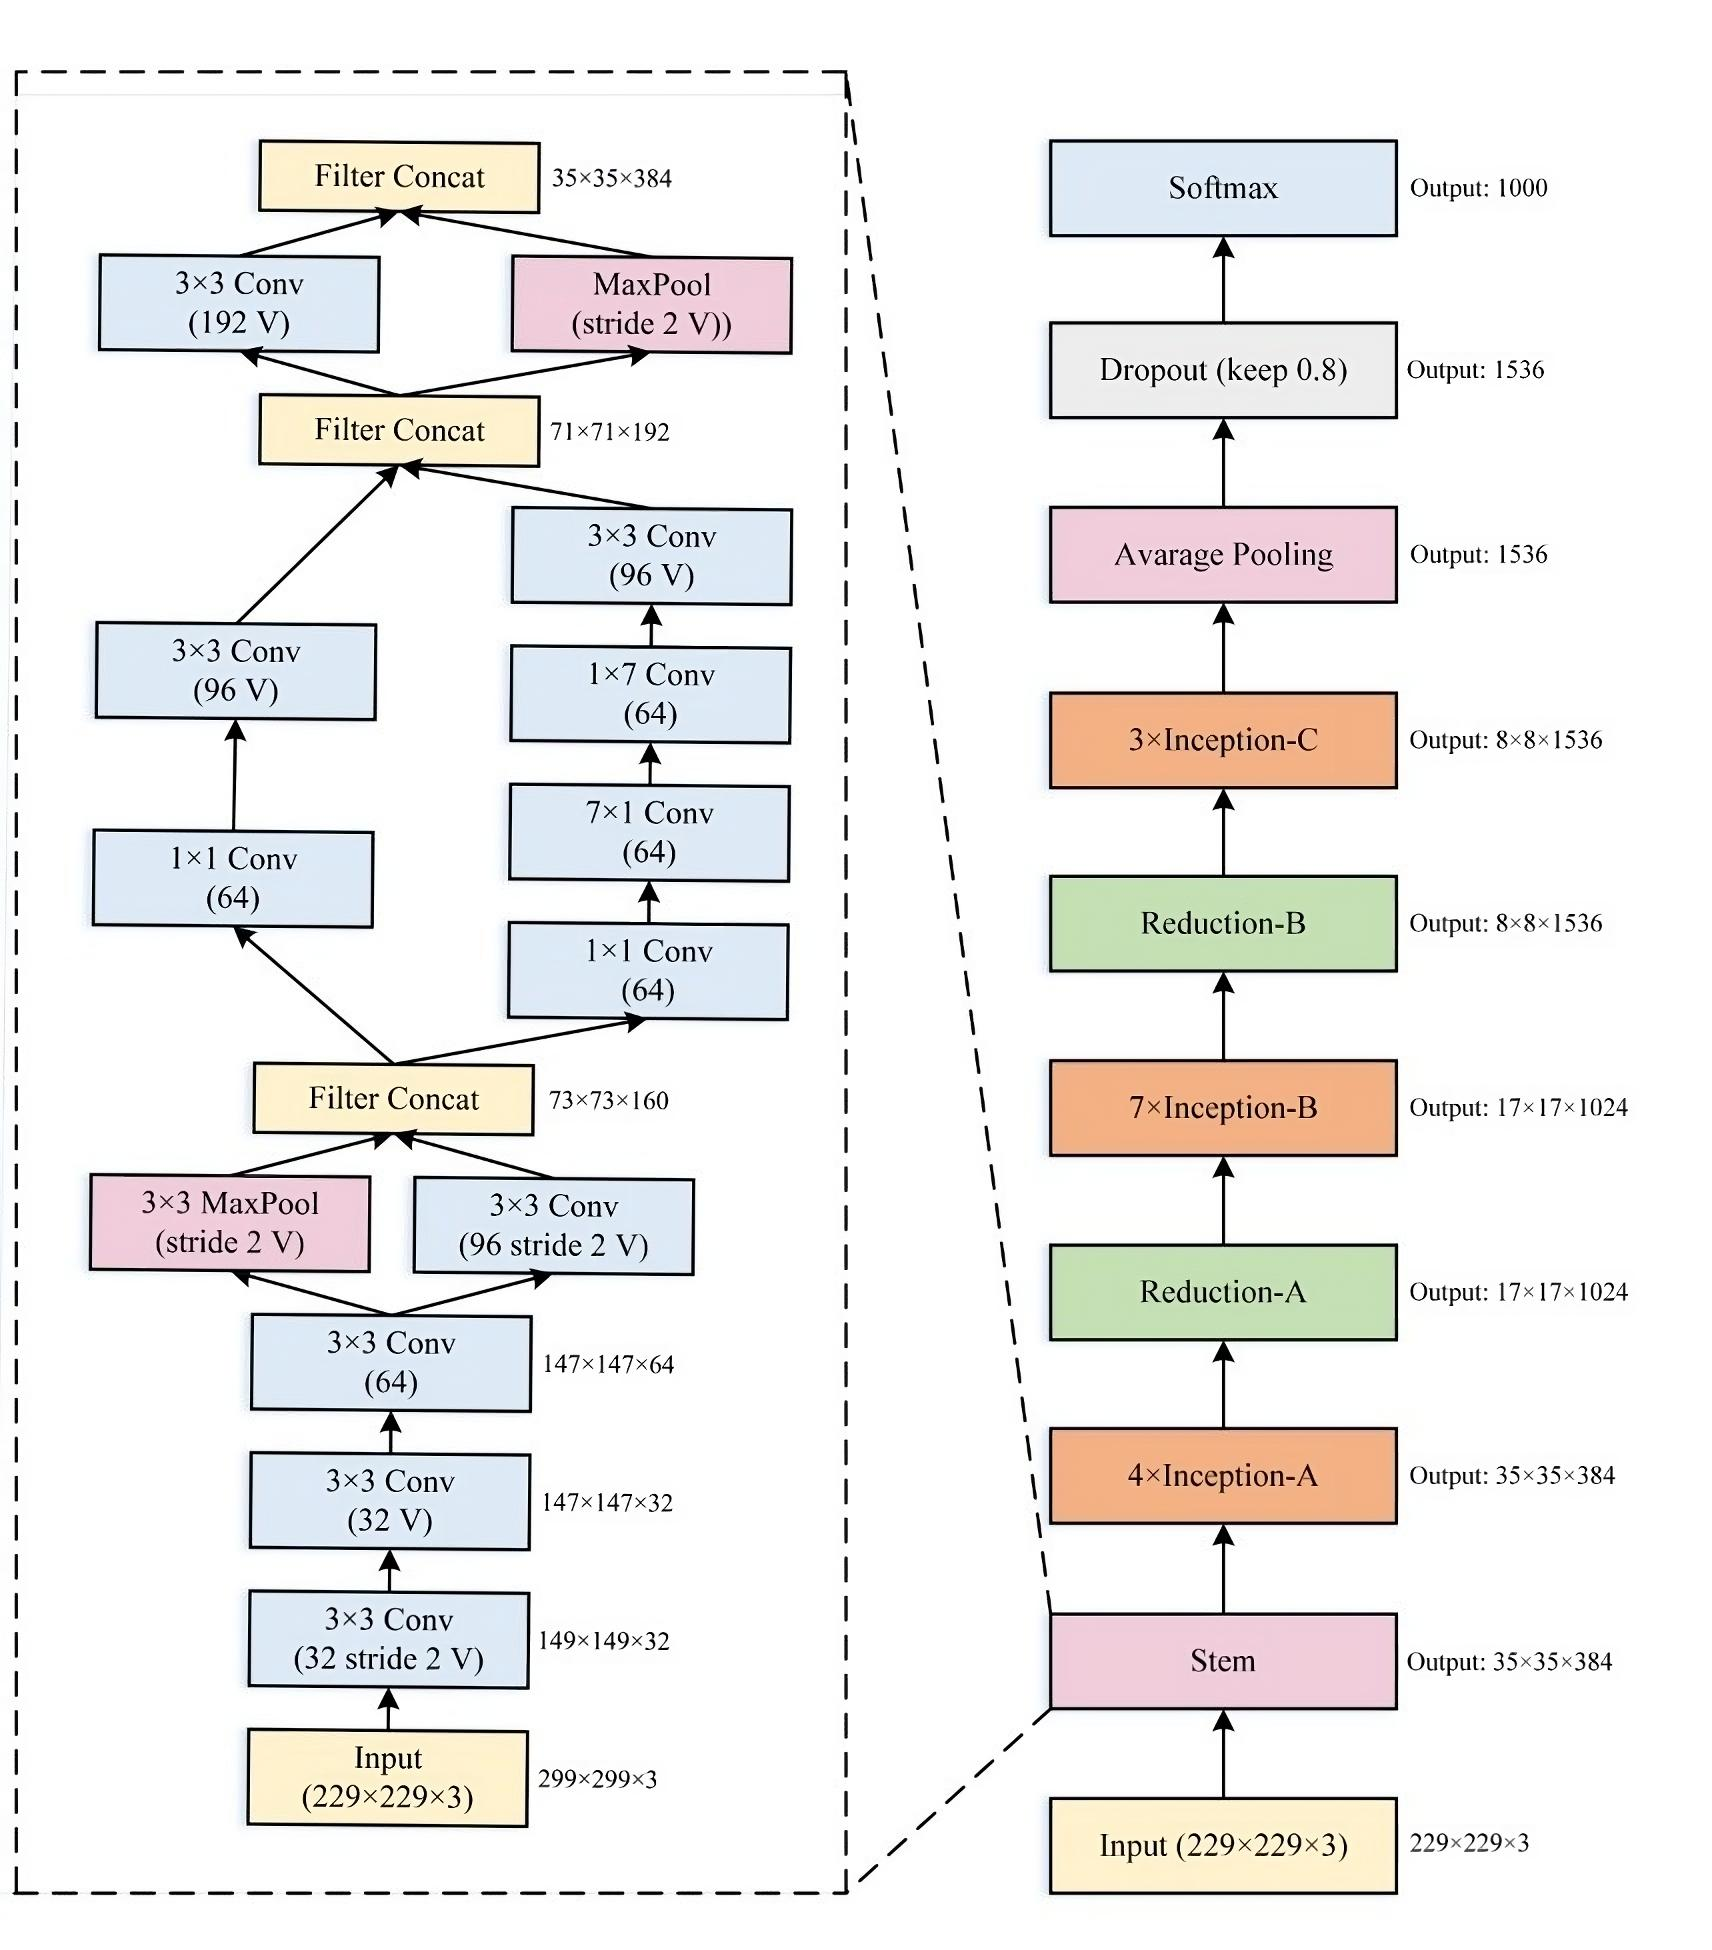
\includegraphics[width=1\textwidth]{2/figures/cnn6.jpeg}
  		\caption{ Arquitectura general de InceptionV4. La parte superior de la imagen es la estructura general, la parte inferior de la
  			La imagen es el tallo de la arquitectura.
  			(\cite{tecnica2})}
  	\end{center}
  \end{figure}
  
  \item \textbf{Residual Learning Networks (ResNet):} En 2015, la red residual profunda ResNet, propuesta por Kaiming He et al., ganó el primer premio en ILSVR2015. A medida que las redes se vuelven más profundas, aumenta el rendimiento de la red, pero simplemente aumentar la profundidad de la red no mejora efectivamente el rendimiento. ResNet aborda este problema mediante conexiones residuales, que permiten que las redes profundas alcancen una alta precisión. En lugar de aprender la asignación deseada directamente, las conexiones residuales ajustan una asignación residual relacionada con la identidad, lo que facilita la optimización y el aprendizaje. Los bloques residuales en ResNet contienen dos capas convolucionales 3x3, seguidas de normalización y activación ReLU, con una conexión directa de entrada al bloque final. Para profundidades mayores, se puede añadir una capa convolucional 1x1 para controlar el número de canales. ResNet ha demostrado ser una contribución significativa al lograr precisión incluso con profundidades mayores, superando a las redes previas.En 2015, ResNet, una red residual profunda propuesta por Kaiming He et al., ganó el primer premio en ILSVR2015. A medida que las redes se vuelven más profundas, el rendimiento aumenta, pero simplemente aumentar la profundidad no garantiza una mejora efectiva. ResNet aborda este desafío mediante conexiones residuales, que permiten a las redes profundas alcanzar altos niveles de precisión. En lugar de aprender directamente la asignación deseada, las conexiones residuales ajustan una asignación residual relacionada con la identidad, lo que facilita la optimización y el aprendizaje. Los bloques residuales en ResNet consisten en dos capas convolucionales 3x3, seguidas de normalización y activación ReLU, con una conexión directa de entrada al bloque final. Para profundidades mayores, se puede añadir una capa convolucional 1x1 para controlar el número de canales. ResNet ha demostrado ser una contribución significativa al lograr una alta precisión incluso con profundidades mayores, superando a las redes anteriores.
  
  \item \textbf{Mejoras de ResNet:}
 ResNet con preactivación: He et al. introdujeron una estructura de preactivación que mejora el rendimiento de ResNet al preactivar la BN y ReLU. Este enfoque permite el entrenamiento exitoso de ResNet con más de 1000 capas, enfatizando la importancia del mapeo de identidad.
 
 Profundidad estocástica: El método de profundidad estocástica, propuesto por Huang et al., elimina ciertas capas durante el entrenamiento, reduciendo significativamente el tiempo de entrenamiento y aumentando la profundidad de ResNet. Este método resulta efectivo incluso con más de 1200 capas, mejorando el error de prueba y el tiempo de entrenamiento en los conjuntos de datos CIFAR-10/100.
 
 Redes Residuales Amplias (WRNs): Para contrarrestar la desaceleración del entrenamiento debido a la disminución de la reutilización de características en redes más profundas, las WRNs introducen bloques de eliminación amplia, ampliando las capas de peso de las unidades residuales originales y agregando eliminación entre ellas. Este enfoque, con menos capas que las ResNets más profundas, reduce el tiempo de entrenamiento y tiene un mejor rendimiento en los conjuntos de datos CIFAR e ImageNet.
 
 ResNeXt: ResNeXt introduce el concepto de "Cardinalidad C", el número de rutas en un bloque, para superar los desafíos de adaptación del conjunto de datos. Aumentar la cardinalidad resulta más efectivo que aumentar la profundidad o el ancho. Las estructuras de convolución agrupada, como en la Figura 18c, son más rápidas y eficientes, formando la base de ResNeXt.
 
 Redes Residuales Dilatadas (DRN): Yu et al. abordan la pérdida de resolución y la reducción de la información de características en el submuestreo al introducir convoluciones dilatadas. Estas convoluciones aumentan el campo receptivo de las capas superiores, compensando la reducción de campos receptivos inducida por la eliminación del submuestreo. DRN logra una precisión significativamente mejorada en la clasificación de imágenes en comparación con ResNet.
 
 Otros modelos: Variantes como la ResNet reducida de Veit et al., Resnet en Resnet (RiR), la técnica DropBlock, Big Transfer (BiT) y NFNet, ofrecen enfoques únicos para mejorar el rendimiento de ResNet. Estos métodos incluyen la eliminación de capas, arquitecturas de doble flujo, eliminación de características y estructuras sin BN, logrando mejoras notables en velocidad de entrenamiento y precisión.
  
  \begin{figure}[H]
  	\begin{center}
  		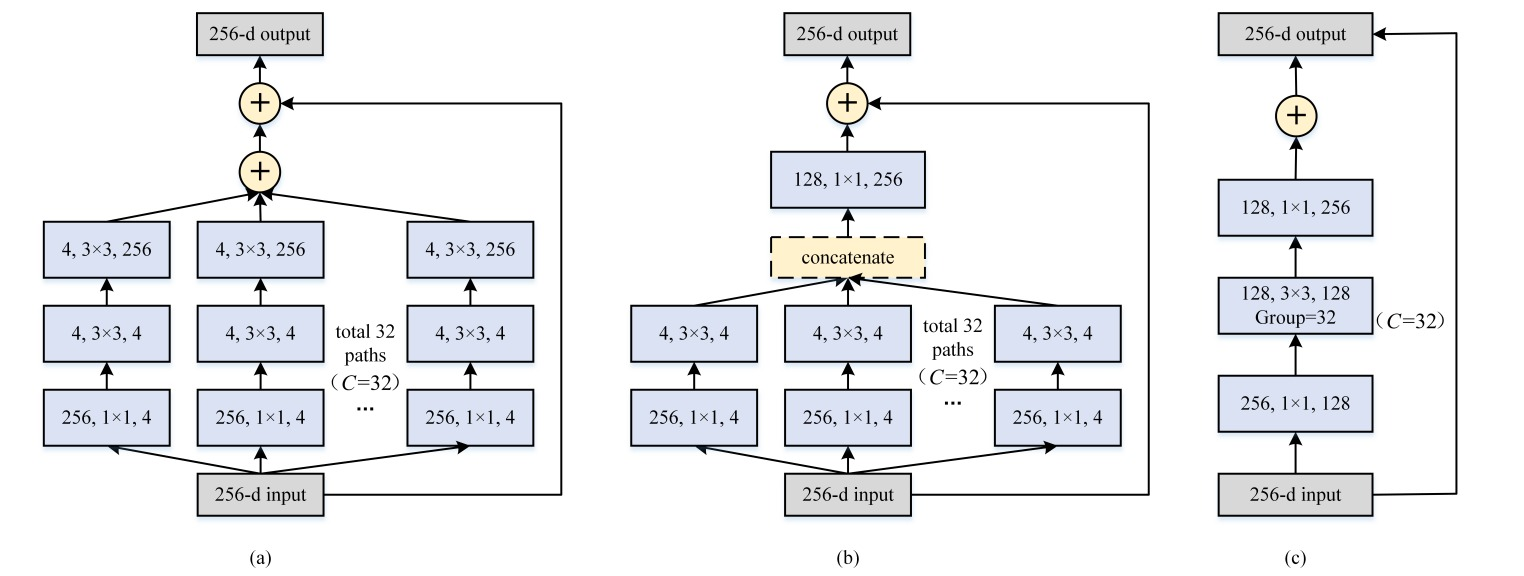
\includegraphics[width=1\textwidth]{2/figures/cnn7.jpeg}
  		\caption{Bloques de construcción equivalentes de ResNeXt.
  			(\cite{tecnica2})}
  	\end{center}
  \end{figure}
  
  \item \textbf{MobileNet V1 to V3:} En 2017, Google presentó MobileNetV1, una red liviana diseñada para dispositivos móviles y embebidos. Utiliza convolución separable en profundidad, que consta de convolución en profundidad y convolución puntual, en lugar de convolución estándar, reduciendo significativamente el costo computacional y los parámetros. MobileNetV1 ofrece dos hiperparámetros, el multiplicador de ancho x y el multiplicador de resolución x, para equilibrar eficazmente el cálculo y la precisión.
  
  En 2018, MobileNetV2 abordó el problema de los parámetros cero en la convolución separable en profundidad al introducir Residuos Invertidos y Cuellos de Botella Lineales. A diferencia del bloque residual estándar, el bloque residual invertido de MobileNetV2 sigue una secuencia de 1 × 1 (expansión) → 3 × 3 → 1 × 1 (compresión). Además, reemplaza el último ReLU con una transformación lineal para evitar la pérdida de información.
  
  En 2019, MobileNetV3 mejoró la eficiencia y precisión al incorporar el bloque SE para atención por canal y la tecnología de Búsqueda de Arquitectura Neural (NAS). El enfoque NAS consciente de la plataforma se utiliza para la búsqueda por bloques para encontrar estructuras globales de red, mientras que NetAdapt ajusta individualmente las capas de manera secuencial. MobileNetV3 también adopta la función de activación h-swish, modificando el sigmoidal de la función swish para mejorar la precisión.
  
    \begin{figure}[H]
  	\begin{center}
  		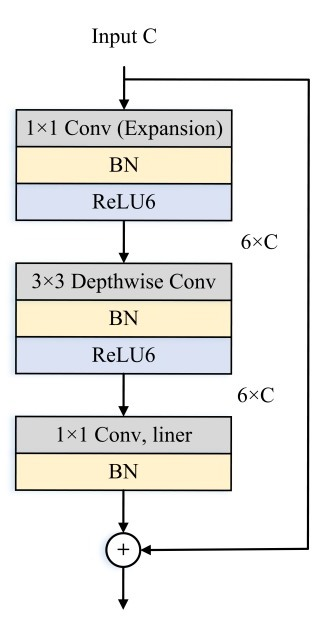
\includegraphics[width=0.6\textwidth]{2/figures/cnn8.jpeg}
  		\caption{  El bloque residual de cuello de botella de MobileNetV2. C es el número de canales y las relaciones de expansión son 6.
  			(\cite{tecnica2})}
  	\end{center}
  \end{figure}
  
  
  \item \textbf{ShuffleNet V1 to V2:}
  
En 2017, ShuffleNetV1, desarrollado por Face++, se enfocó en plataformas móviles como drones, robots y teléfonos inteligentes. Utiliza convolución Pointwise Group y Channel Shuffle para mejorar el bloque residual. La convolución Pointwise Group resuelve el problema de los canales limitados debido a convoluciones costosas, mientras que Channel Shuffle aborda la pérdida de información entre grupos de canales en bloques de convolución de grupo. La unidad ShuffleNet (stride = 1) reemplaza la primera convolución 1 × 1 con convolución de grupo pointwise seguida de una operación de mezcla de canales. La unidad ShuffleNet (stride = 2) agrega un GAP de 3 × 3 a la ruta de acceso directo y reemplaza la concatenación de canales con una suma de elementos. MobileNetV1 experimentó con diferentes números de grupos para convoluciones y escalas para el número de filtros.

En 2018, ShuffleNetV2 optimizó la velocidad y precisión considerando la complejidad computacional, el costo de acceso a la memoria y las características de la plataforma. Cuatro directrices principales surgieron de los experimentos: el ancho de canal igual minimiza el costo de acceso a la memoria; la convolución de grupo excesiva aumenta este costo; la fragmentación de la red reduce el paralelismo y las operaciones elemento a elemento tienen una alta relación MAC/FLOPs. La unidad ShuffleNetV2 evita violar estas directrices para mejorar la eficiencia.
      \begin{figure}[H]
  	\begin{center}
  		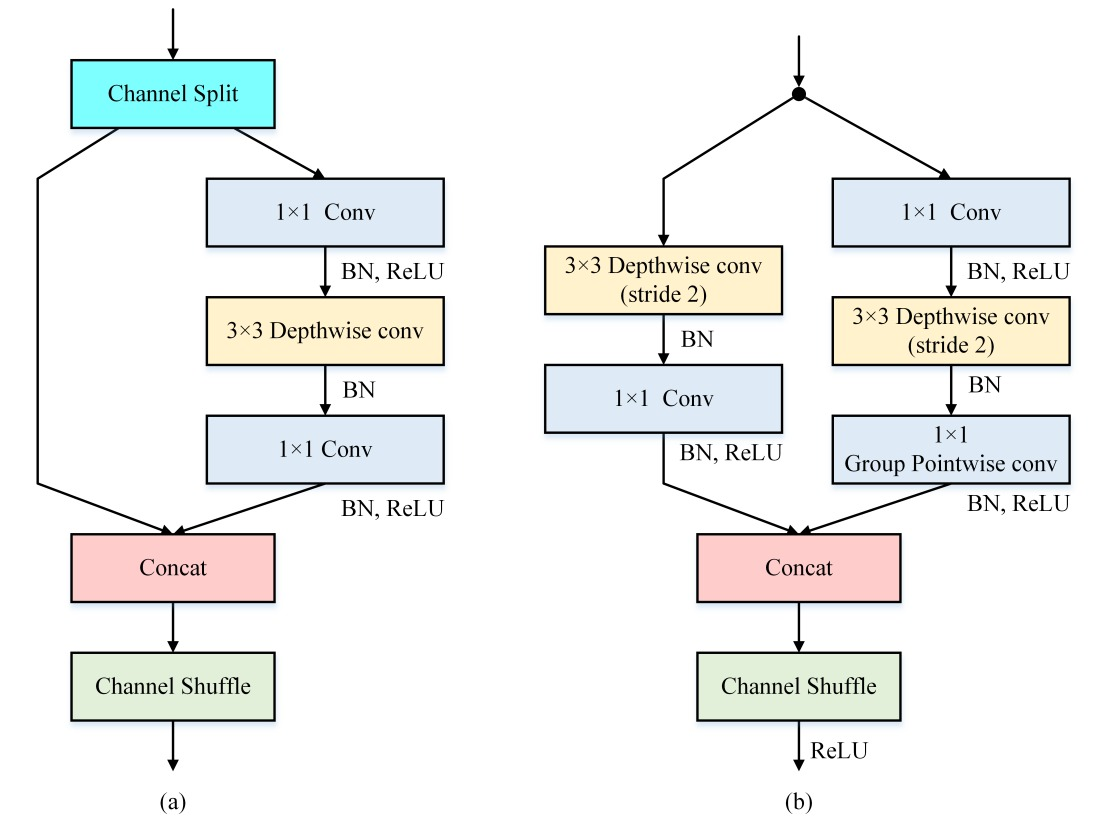
\includegraphics[width=1\textwidth]{2/figures/cnn9.jpeg}
  		\caption{  El bloque residual de cuello de botella de MobileNetV2. C es el número de canales y las relaciones de expansión son 6.
  			(\cite{tecnica2})}
  	\end{center}
  \end{figure}
  
  \item \textbf{Data Augmentation:} as CNN a menudo enfrentan el riesgo de sobreajuste debido a datos limitados. Las técnicas tradicionales de aumento de datos incluyen una colección de métodos, como voltear, cambiar el espacio de color, recortar, rotar, trasladar e inyectar ruido, que pueden mejorar los atributos y el tamaño del conjunto de datos de entrenamiento. Además, tienen el potencial de mejorar significativamente la generalización de los modelos de DL. El aumento de datos automatizado tiene el potencial de abordar algunas debilidades de los métodos tradicionales de aumento de datos, ya que entrenar un modelo CNN con una política de aumento de datos aprendida puede mejorar significativamente la precisión, la robustez del modelo y el rendimiento en el aprendizaje semi-supervisado para la clasificación de imágenes. La técnica de Aumento de Datos de Muestra Mixta (MSDA) consiste en mezclar aleatoriamente dos muestras de entrenamiento y sus etiquetas según una cierta proporción, lo que no solo puede reducir la identificación errónea de algunas muestras difíciles, sino también mejorar la robustez del modelo y hacerlo más estable durante el entrenamiento.
   \end{itemize}
 \subsubsection{Conclusiones} 
Esta revisión abarca no solo los modelos convencionales de CNN, sino también métodos mixtos y estrategias de entrenamiento, destacando puntos clave en la clasificación de imágenes.

Los modelos clásicos de CNN (2012-2017) sentaron las bases para el diseño estructural actual. La integración del mecanismo de atención en las CNN, como los bloques SE, mejora su rendimiento. Las redes para plataformas móviles son más pequeñas y eficientes, aprovechando al máximo los recursos limitados. La elección de hiperparámetros es crucial, y la búsqueda NAS facilita el diseño de redes de alto rendimiento. El aprendizaje por transferencia y el aumento de datos mejoran las predicciones y el rendimiento.

Los modelos livianos sacrifican precisión por eficiencia, y aún se explora su uso en sistemas limitados. El campo de NLP ha avanzado más en el aprendizaje semi-supervisado y no supervisado.

Futuras direcciones incluyen la combinación de convolución y Transformer, como en la red CoAtNet, y la revisión de componentes convencionales de CNN, que podría llevar a avances significativos.
 \subsection{Vision Computer}
 
 Según \cite{alonso2016vision}, la Visión por computadora también conocido como visión artificial es otra rama importante de la IA que desempeña la tarea de dotar al computador la función de captar y comprender una imagen con el objetivo de emular el proceso que realizan los humanos. A pesar de tener menos tiempo a comparación con las otras, desempeña una función básica, primordial y compleja del reconocimiento. Esta es capaz de aprender y reconocer formas para luego darles una clasificación correctamente.
 Posee funciones como el reconocimiento donde en la imagen se indaga un objeto singular o reconocer diferentes instancias de una categoría genérica donde se hace dicho reconocimiento de la instancia. Este reconocimiento está asignado para categorizar diferentes clases a los objetos, el instrumento que ejecuta este procedimiento se llama clasificador.  Otro método es la representación de objetos, que se trata acerca de que los objetos sean identificados mediante segmentación de imágenes, pueden ser subdivididos en múltiples agrupaciones, desde el punto de agrupación, se provee de características comunes que tienen los objetos entre sí. El objeto medido según sus características es denominado patrón. Por último, tenemos al seguimiento de objetos en tiempo real, que consiste en que las técnicas o algoritmos de seguimiento estimen el movimiento de objetivo en el plano de la imagen mientras se da un contexto en movimiento, para eso el sistema coloca etiquetas fijas al objeto o los objetos a continuar durante continuidad de imágenes. La dificultad de esta técnica radica en los cambios inesperados en el movimiento, como la alteración en los aspectos de patrones, tal como de la escena, el propio objeto y las oclusiones entre objetos \parencite{alonso2016vision}.
 
 \subsection{Vision Transformer: Explainability of Vision Transformers: A Comprehensive Review and New Perspectives \citep*{tecnica1}}
 Los transformers han sido importantes en el procesamiento del lenguaje y, recientemente, se han destacado en la visión por computadora. Aunque su funcionamiento interno no se comprende completamente, la explicabilidad es crucial. Este estudio revisa métodos de explicabilidad para transformers visuales, propone una taxonomía y ofrece criterios de evaluación y herramientas. También señala áreas no exploradas que podrían mejorar la explicabilidad y sugiere futuras investigaciones.
 
 \subsubsection{Introducción}
 La Inteligencia Artificial (IA) ha experimentado avances notables en los últimos años, principalmente impulsada por el éxito de las Redes Neuronales Profundas (DNNs) en una amplia gama de aplicaciones, como el diagnóstico médico, las aplicaciones financieras, las evaluaciones de riesgos y la generación de imágenes y videos. Estos logros han sido significativos en términos de rendimiento y precisión en diversas tareas, sin embargo, la aplicación práctica de las DNNs sigue siendo limitada debido a su naturaleza opaca y la falta de transparencia en su toma de decisiones.
 
 La opacidad de las DNNs plantea preocupaciones importantes en términos de confiabilidad y seguridad, ya que los usuarios y los responsables de la toma de decisiones pueden tener dificultades para comprender por qué un modelo ha llegado a una determinada conclusión o recomendación. Esto es particularmente problemático en áreas donde las decisiones basadas en IA pueden tener un impacto significativo en la vida de las personas, como la salud y la justicia. La falta de transparencia también puede ocultar sesgos y errores en los modelos, lo que socava aún más la confianza en su uso.
 
 Para abordar estos desafíos, ha surgido el campo de la Inteligencia Artificial Explicable (XAI), cuyo objetivo es mejorar la comprensión y la transparencia de los modelos de IA. La XAI busca proporcionar explicaciones claras y comprensibles sobre cómo se toman las decisiones por parte de los modelos de IA, permitiendo a los usuarios entender y confiar en sus resultados. Al comprender cómo funciona un modelo y por qué toma ciertas decisiones, los usuarios pueden evaluar mejor su fiabilidad y corregir posibles sesgos o errores.
 
 En este contexto, los transformers, modelos basados en atención, han surgido como una alternativa poderosa a las arquitecturas de redes neuronales convolucionales (CNNs) tradicionales en áreas como el Procesamiento del Lenguaje Natural (NLP) y la Visión por Computadora (CV). Los transformers han demostrado ser altamente efectivos para capturar relaciones a largo plazo en datos secuenciales, lo que los hace adecuados para tareas que requieren un procesamiento de contexto complejo.
 
 En particular, los Vision Transformers (ViT) aplican la arquitectura de transformers a la tarea de visión por computadora, lo que ha llevado a avances significativos en tareas como el reconocimiento de imágenes, la detección de objetos y la segmentación de imágenes. Los ViT han demostrado resultados comparables e incluso superiores a los obtenidos con CNNs en algunas aplicaciones.
 
 Sin embargo, a pesar de su éxito, la comprensión y la explicabilidad de los transformers, especialmente en el contexto de la visión por computadora, siguen siendo áreas de investigación activa. Se necesitan métodos y técnicas robustas para explicar las decisiones tomadas por estos modelos, así como herramientas y marcos para evaluar y comparar sus explicaciones. Al mejorar la explicabilidad de los transformers, podemos fortalecer la confianza en su uso y abrir nuevas oportunidades para aplicaciones prácticas en una variedad de campos.
 
\subsubsection{ Arquitectura de Vision Transformer}
Los Vision Transformers (ViTs) aprovechan los avances de los transformers en NLP para aplicaciones visuales. Utilizan bloques de transformers que permiten integrar información global en toda la imagen mediante auto-atención. Las imágenes se representan como secuencias de tokens, con una capa de incrustación de parches para dividirlas en parches. Estos parches se aplanan y se tratan como tokens, luego se transforman en vectores de características. Para la clasificación, se agrega un token de clasificación. La red ViT también incluye otros componentes como una activación GELU, normalización de capa y conexión residual.Se puede encontrar una ilustración de la arquitectura ViT en la Figura 7.
  \begin{figure}[H]
  	\begin{center}
  		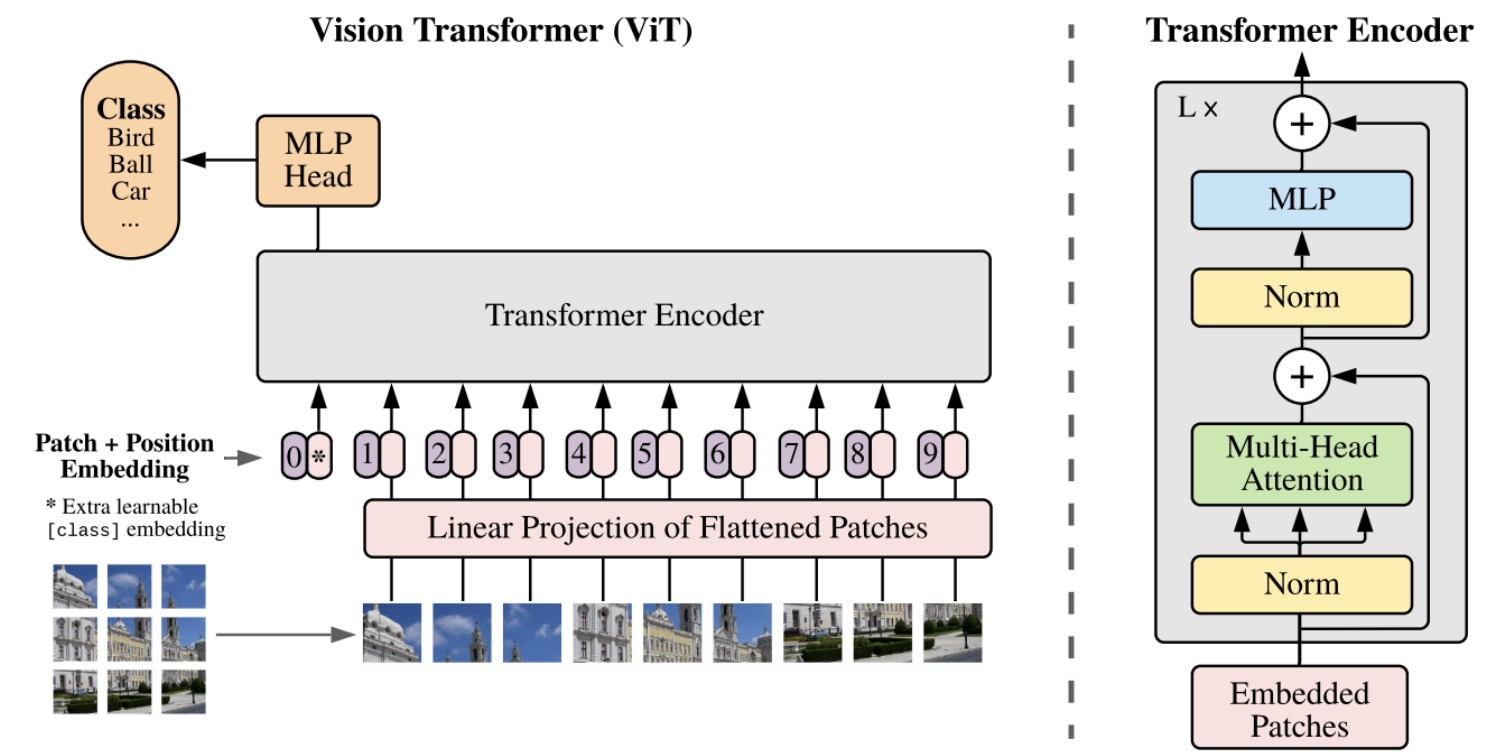
\includegraphics[width=1\textwidth]{2/figures/vt1.jpeg}
  		\caption{Arquitectura de Vision Transformer (\cite{tecnica1})}
  	\end{center}
  \end{figure}
 
 \subsubsection{ Explicacion y métodos para Visual Transformer} 
 Tras los trabajos innovadores presentados basados en transformers visuales para diversos dominios de visión por computadora, han surgido múltiples enfoques para mejorar la explicabilidad de estas redes. Sin embargo, se necesita una encuesta exhaustiva para comprender mejor estos métodos e identificar áreas de mejora. Con un enfoque en la tarea de clasificación, esta sección presenta una visión general de las técnicas de explicabilidad existentes para transformers visuales. Para proporcionar una visión clara, categorizamos y resumimos estos métodos en cinco grupos distintos según sus procedimientos de trabajo, motivaciones y características estructurales, como se ilustra en la Figura 8.
    \begin{figure}[H]
  	\begin{center}
  		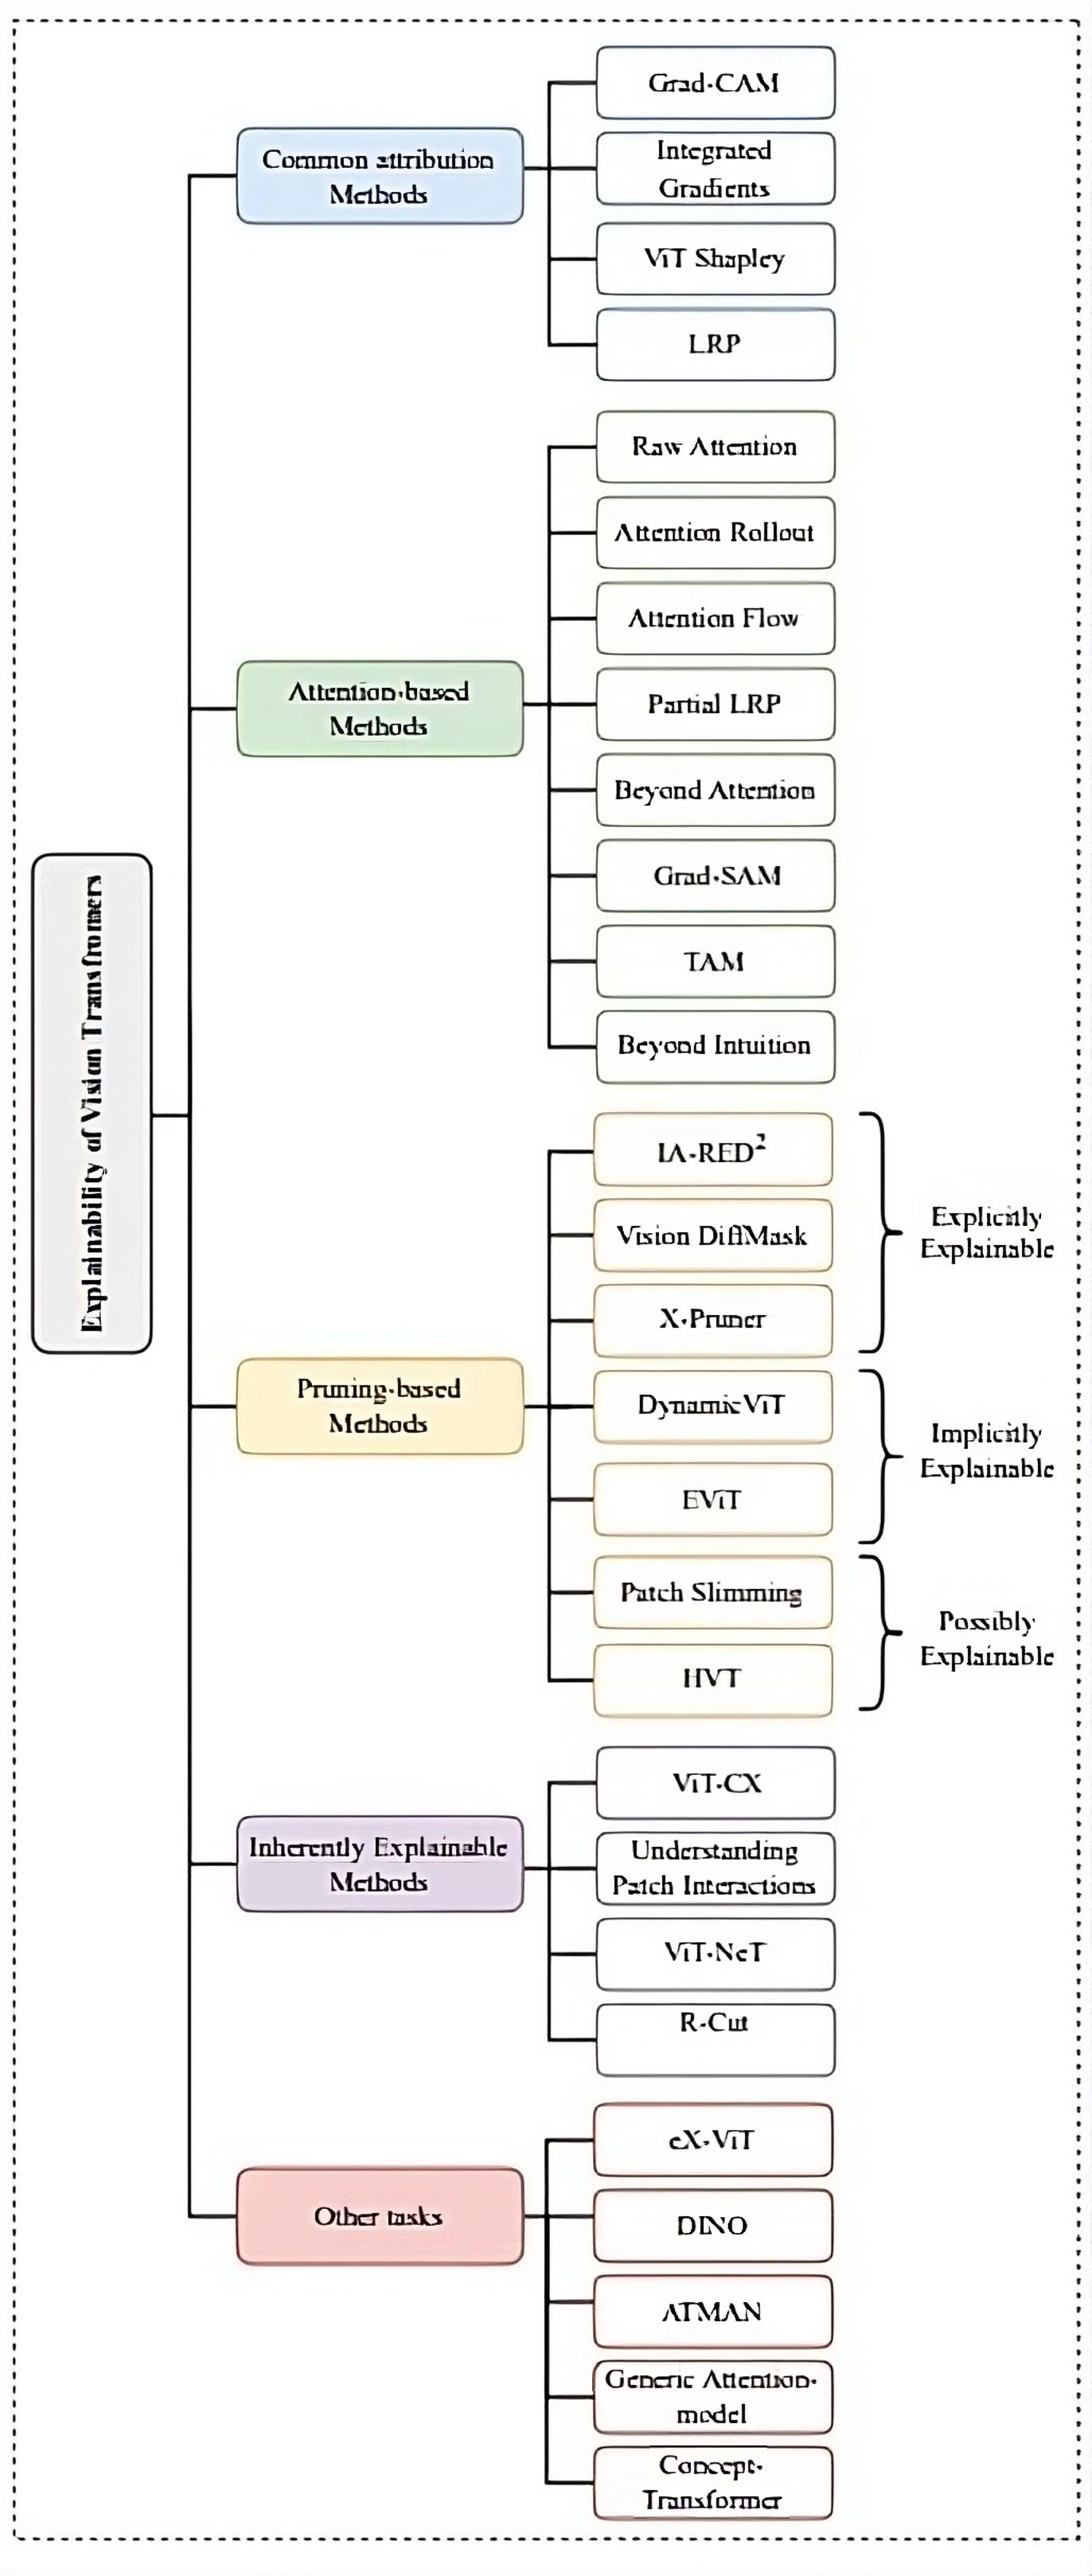
\includegraphics[width=0.6\textwidth]{2/figures/vt2.jpeg}
  		\caption{ Taxonomía de los métodos de explicabilidad para
  			Transformadores de visión (\cite{tecnica1})}
  	\end{center}
  \end{figure}
  
   \subsubsection{ Métodos basados en atención}
  Los métodos basados en atención aprovechan el mecanismo de atención de los modelos para identificar y priorizar las partes más relevantes de una secuencia de entrada. Muchos enfoques existentes se centran en utilizar los pesos de atención o el conocimiento codificado en ellos para explicar el comportamiento del modelo. En aplicaciones basadas en visión, la visualización de los pesos de atención puede ser útil para identificar patrones de atención, aunque puede volverse menos confiable a medida que la red crece más profunda y más compleja. Para superar estos desafíos, se han introducido dos métodos: "Attention Rollout" y "Attention Flow", que cuantifican el flujo de información y aproximan la atención a los tokens de entrada de manera más holística. Estos métodos tienen sus limitaciones, por lo que se han desarrollado enfoques adicionales, como "GradSAM" y "Transition Attention Maps" (TAM), que aplican funciones como gradientes a los pesos de atención para mejorar la explicación de las predicciones del modelo. Además, el marco "Beyond Intuition" propone una aproximación novedosa para aproximarse a las contribuciones de los tokens, operando en dos etapas: percepción de atención y retroalimentación de razonamiento.
  
\begin{table}[htbp]
	\centering
	\caption{Methods for Attention-based Class-specific Multi-modality}
	\label{tab:methods}
	\begin{tabular}{llllll}
		\toprule
		Method & Attention & Class-specific & Multi-modality & Backbone & Date \\
		\midrule
		Raw Attention & Yes & No & No & VIT, DEIT & 2017 \\
		Attention Rollout & Yes & No & No & VIT, DEIT & 2020 \\
		Attention Flow & Yes & No & No & VIT, DEIT & 2020 \\
		Partial LRP & Yes & No & No & VIT & 2019 \\
		Grad-SAM & Yes & Yes & No & VIT & 2021 \\
		Beyond Attention & Yes & Yes & Yes & VIT & 2021 \\
		TAM & Yes & Yes & No & VIT, DEIT & 2021 \\
		Beyond Intuition & Yes & Yes & Yes & BERT, VIT, CLIP & 2023 \\
		\bottomrule
	\end{tabular}
\end{table}
  
       \begin{figure}[H]
  	\begin{center}
  		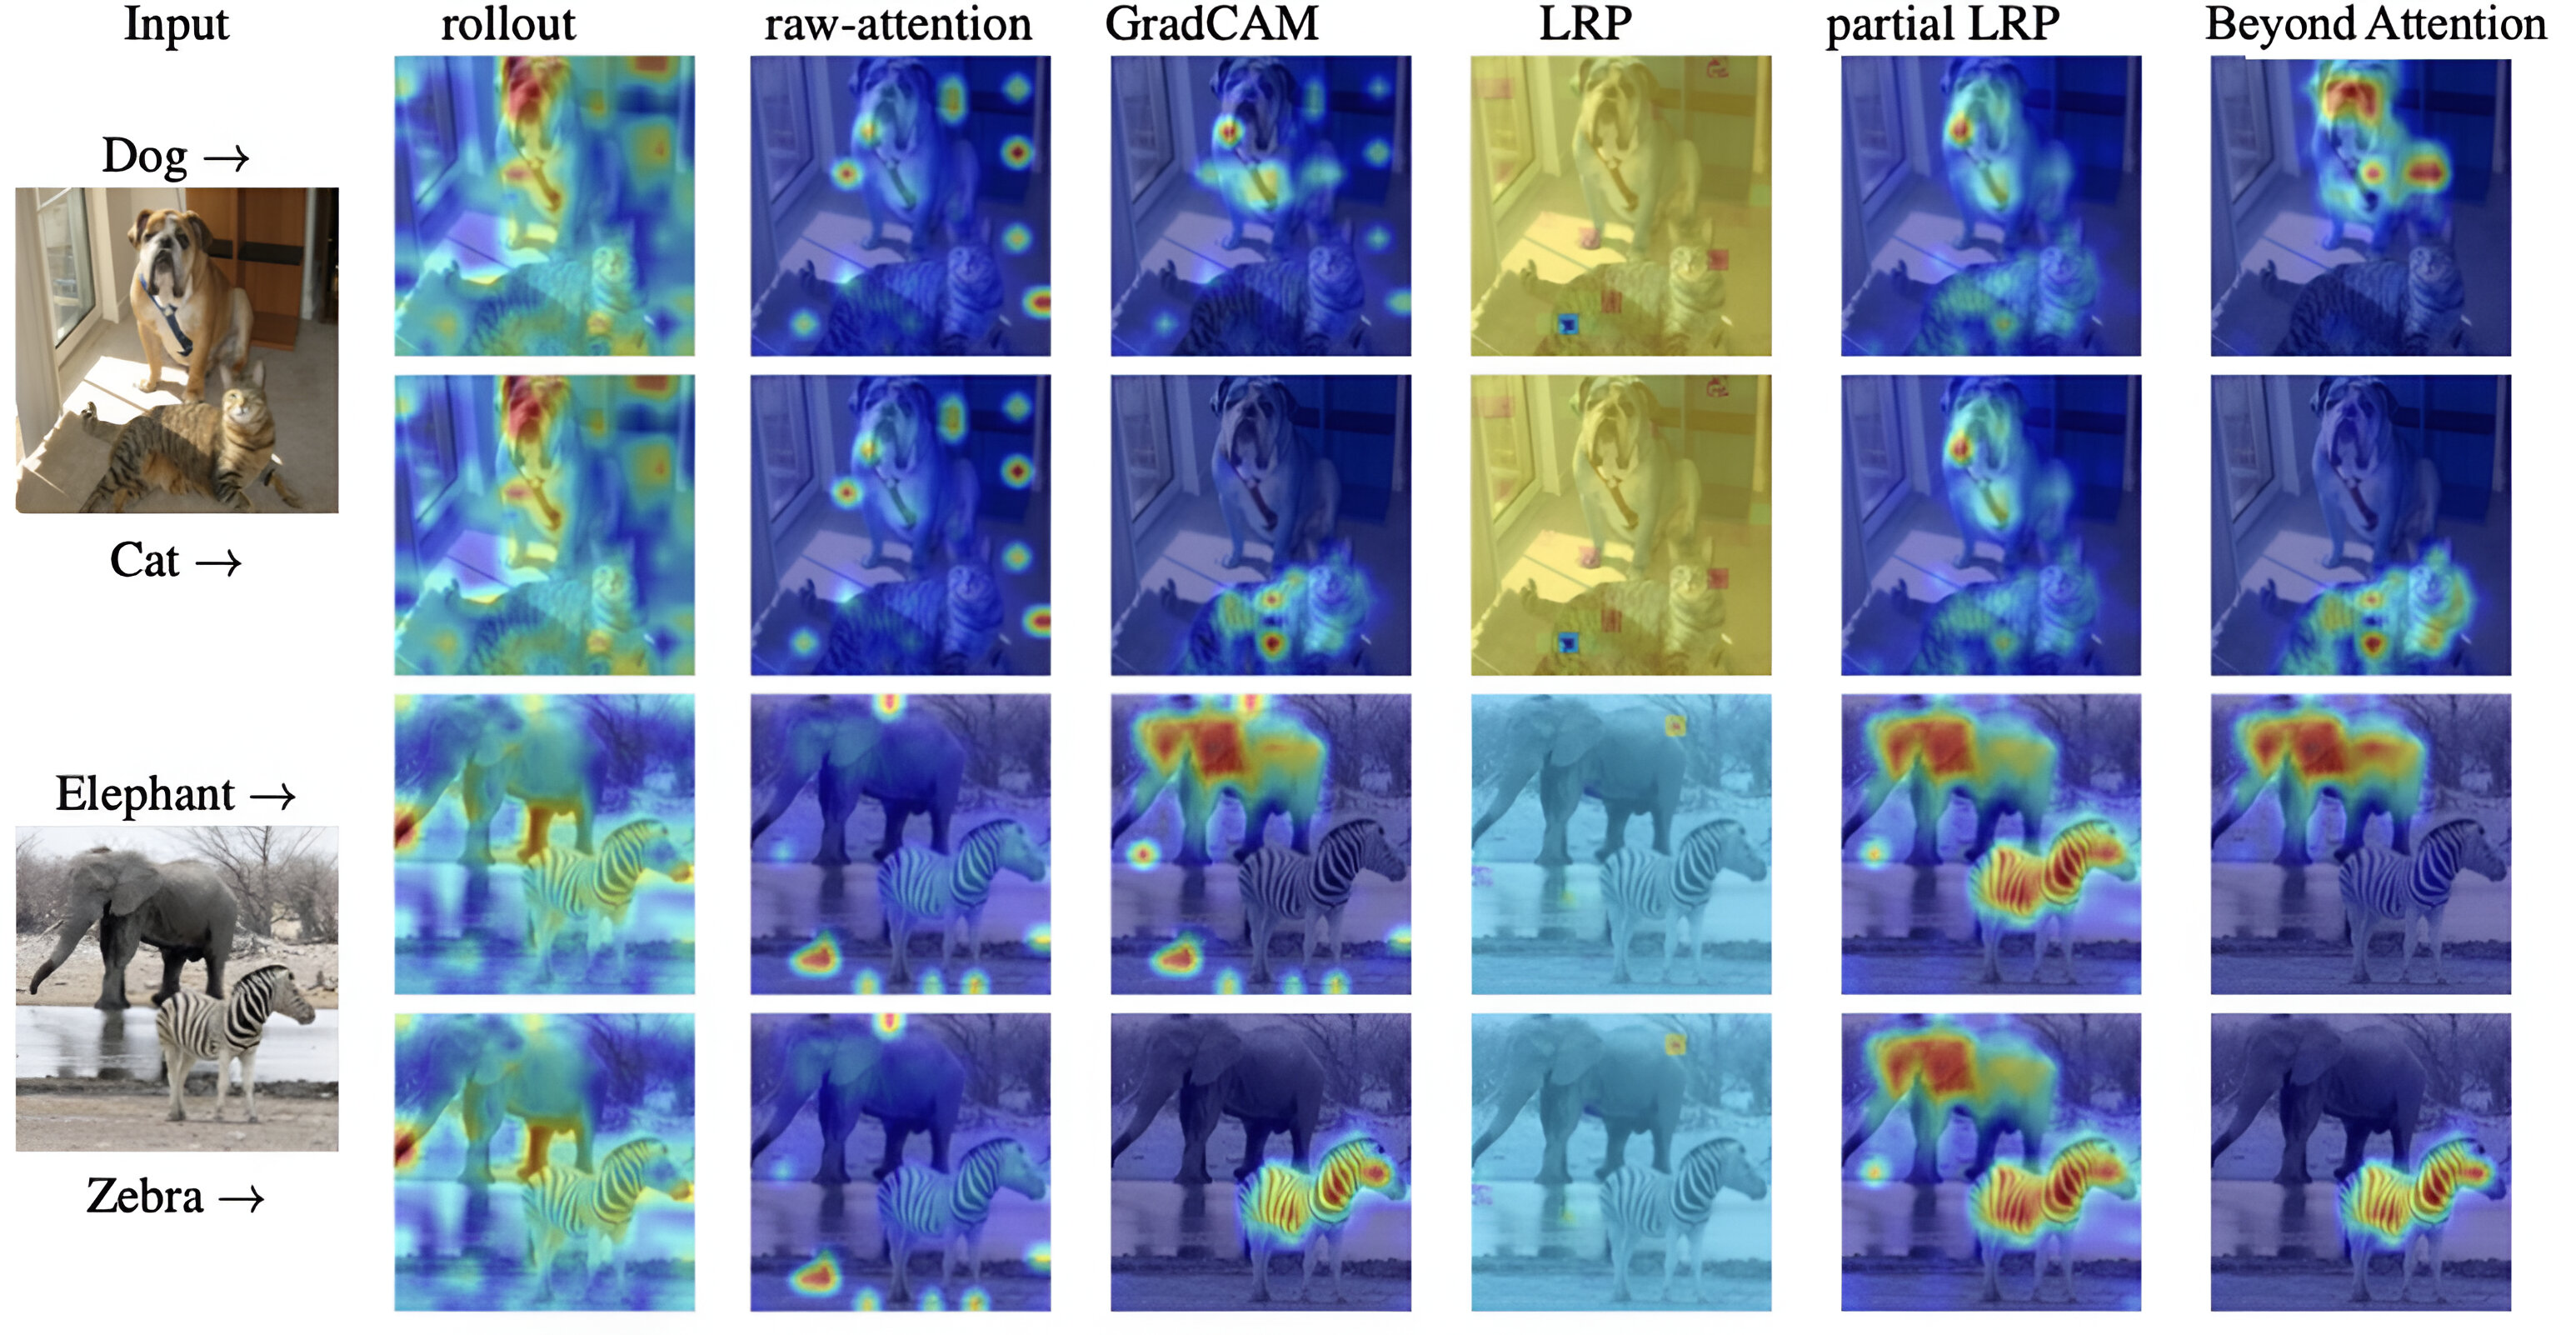
\includegraphics[width=1\textwidth]{2/figures/vt4.jpeg}
  		\caption{ Visualizaciones específicas de clase de varios métodos basados en la atención, para cada imagen se pueden ver resultados de dos clases diferentes(\cite{tecnica1})}
  	\end{center}
  \end{figure}
  
\subsubsection{ Métodos basados en la poda} 
Los métodos basados en poda son una poderosa herramienta utilizada para optimizar la eficiencia y complejidad de los transformers. Estos métodos intentan eliminar elementos redundantes o poco informativos como tokens, parches, bloques o cabezas de atención de las redes. Algunos de estos métodos están explícitamente desarrollados con fines de explicabilidad, mientras que otros se centran principalmente en mejorar la eficiencia y no tienen como objetivo específico la explicabilidad. Sin embargo, estudios indican que las técnicas del segundo grupo también pueden impactar positivamente la explicabilidad del modelo. Se pueden categorizar los métodos de poda basados en ViT en tres grupos: métodos explícitamente explicables, implícitamente explicables y posiblemente explicables.

Entre los métodos de poda explícitamente explicables, hay varios enfoques notables que buscan proporcionar modelos menos complejos y más interpretables. Por ejemplo, el método IA-RED2 busca encontrar el equilibrio perfecto entre eficiencia e interpretabilidad al eliminar dinámicamente los parches menos informativos, lo que resulta en una velocidad significativamente mayor con una pérdida mínima de precisión. Otro método, X-Pruner, está diseñado específicamente para podar unidades menos significativas, logrando importantes ahorros computacionales sin perder precisión.

Por otro lado, los métodos de poda implícitamente explicables, como el marco DynamicViT, están diseñados principalmente para mejorar la eficiencia de la red, pero también pueden mejorar la explicabilidad al localizar las partes críticas de la imagen que contribuyen más a la clasificación. EViT es otro enfoque innovador que reorganiza los tokens de una imagen basándose en el concepto de atención, manteniendo los tokens más relevantes mientras fusiona los menos atentos en un solo token, lo que reduce los costos computacionales sin comprometer la precisión del modelo. Estos métodos mejoran la interpretabilidad y ofrecen una comprensión más clara de las decisiones del modelo.   

\begin{table}[H]
	\centering
	\caption{ Comparacion de metodos de poda basados en DeiT-S Touvron en 2021 en el conjunto de datos ImageNet}
	\label{tab:pruning_comparison}
	\begin{tabular}{lccc}
		\toprule
	Método de poda & GFLOPs $\downarrow$ (\%) & TOP-1 Exactitud $\downarrow$ (\%) & Rendimiento $\uparrow$ (\%) \\
		\midrule
		IA-RED2        & --                        & 0.7                               & 46                            \\
		DynamicViT     & 37                        & 0.5                               & 54                            \\
		EViT           & 35                        & 0.3                               & 50                            \\
                           
		HVT            & 47.8                      & 1.8                               & --                            \\
		\bottomrule
	\end{tabular}
\end{table}


Los métodos posiblemente explicables son enfoques adicionales de poda que, aunque inicialmente no se diseñaron para mejorar la interpretabilidad de ViT, podrían ofrecer un potencial para investigar su impacto en la explicabilidad de los modelos. Por ejemplo, Patch Slimming es un algoritmo novedoso que acelera ViTs al dirigirse a los parches redundantes en las imágenes de entrada, lo que potencialmente destaca características visuales importantes y mejora la interpretabilidad. Otro enfoque, Hierarchical Visual Transformer (HVT), mejora la escalabilidad y el rendimiento de ViTs al reducir gradualmente la longitud de la secuencia a medida que aumenta la profundidad del modelo. Aunque estos métodos se han evaluado principalmente en términos de eficiencia, existe una brecha significativa en la literatura en cuanto a la evaluación de su explicabilidad. En contraste, los métodos inherentemente explicables, como ViT-CX, se centran en desarrollar modelos que puedan explicarse a sí mismos, utilizando herramientas interpretables como mapas de saliencia para proporcionar explicaciones más significativas.

   \begin{figure}[H]
	\begin{center}
		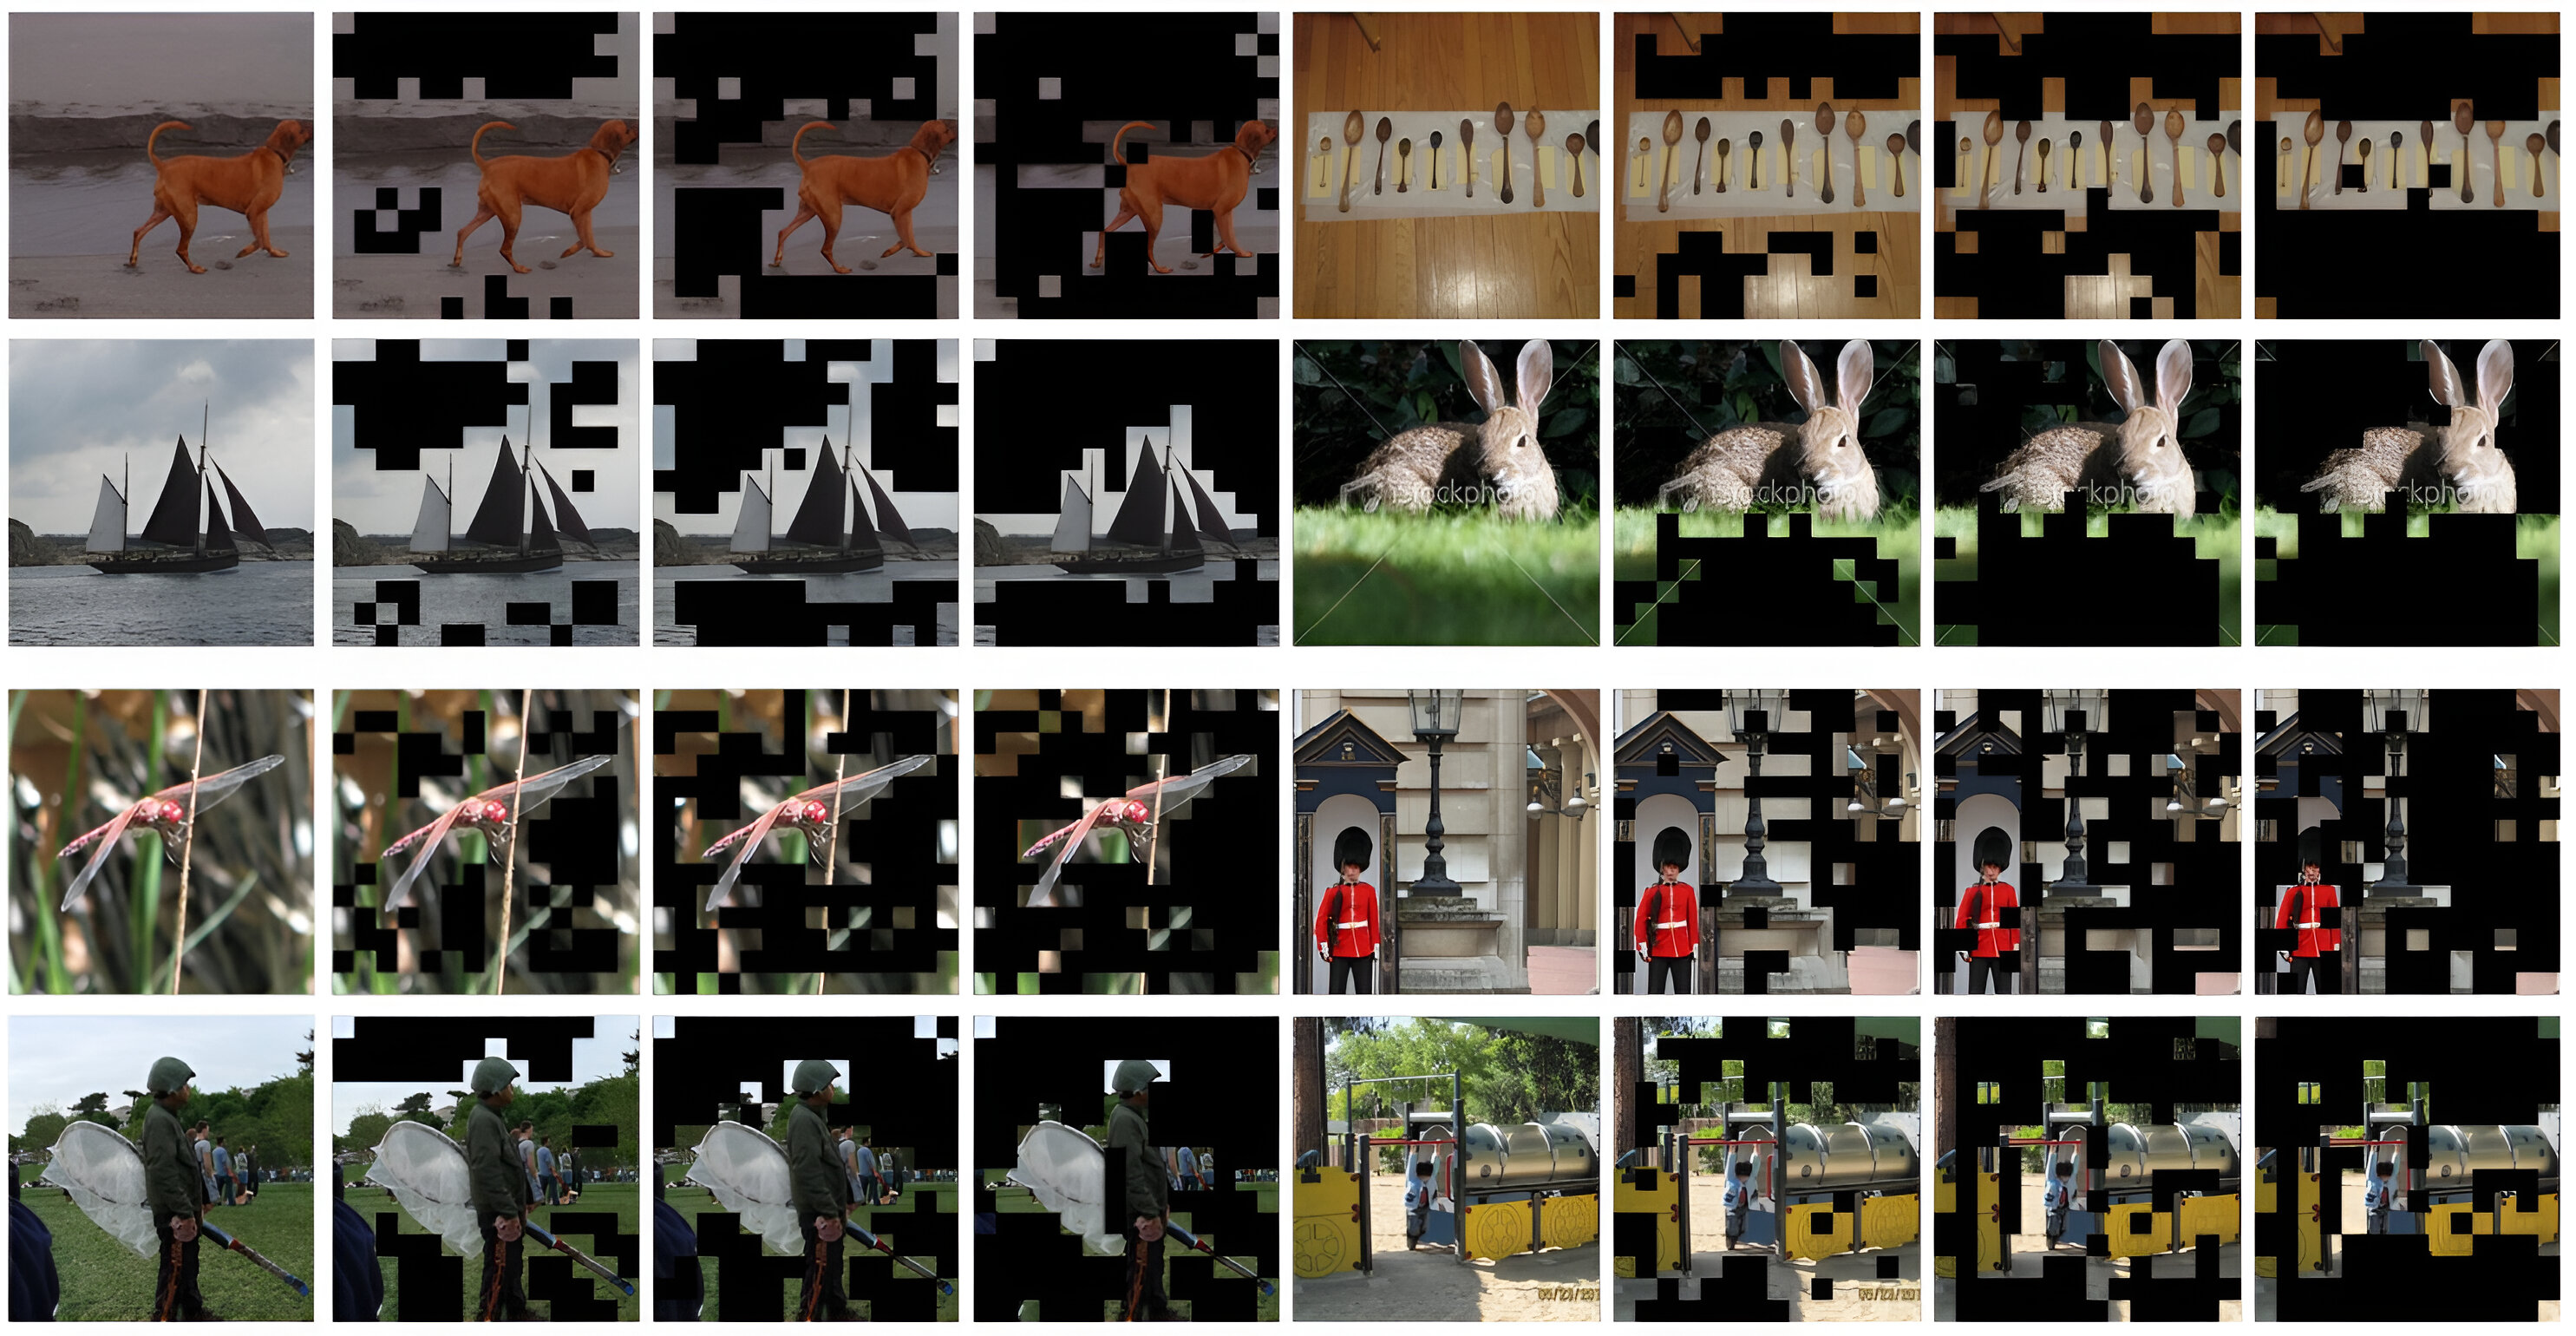
\includegraphics[width=1\textwidth]{2/figures/vt6.jpeg}
		\caption{Visualización de tokens desatentos en EViT-DeiT-S con 12 capas; Se puede ver que las fichas de falta de atención se fusionan gradualmente (como se representa mediante áreas enmascaradas) o se eliminan, mientras que las fichas más informativas se conservan. Esto permite a los ViT centrarse en tokens específicos de clase en imágenes, lo que conduce a una mejor interpretabilidad(\cite{tecnica1})}
	\end{center}
\end{figure}


 \subsubsection{Evaluación de explicación}
 En secciones anteriores, presentamos varias técnicas de explicación desarrolladas específicamente para aplicaciones basadas en ViT. Sin embargo, evaluar qué tan bien estas técnicas representan el proceso de razonamiento de un modelo presenta diferentes desafíos. Para abordar esta preocupación, la literatura sugiere una serie de criterios evaluativos, que ayudan a seleccionar y diseñar la técnica de explicabilidad más apropiada. A continuación, se resumen estos criterios:
 \begin{itemize}
 	\item \textbf{Deletion and Insertion:} Se utilizan para evaluar la fidelidad de un mapa de saliencia al modelo objetivo. Calculan cómo el mapa de saliencia identifica los píxeles más influyentes para la predicción del modelo.
 	\item \textbf{Effective Complexity:} Evalúa el número de atribuciones que superan un umbral, indicando la importancia o insignificancia de las características correspondientes.
 	
 	\item \textbf{Faithfulness:} Método para evaluar la calidad de las atribuciones de características sin intervención humana, midiendo cuán precisamente las atribuciones de características se alinean o correlacionan con las predicciones del modelo.
 	
 	\item \textbf{(In)fidelity:} Se utiliza para evaluar qué tan bien una explicación captura los cambios en las predicciones de un modelo cuando la entrada sufre perturbaciones significativas.
 	
 	\item \textbf{Intersection over Union (IoU) test:} Métrica estándar para evaluar el rendimiento de los detectores y seguidores de objetos, que también se ha utilizado para evaluar métodos de explicabilidad midiendo la superposición entre los mapas de explicabilidad predichos y las cajas delimitadoras de la verdad terrenal de los objetos de interés.
 	
 	\item \textbf{Perturbation Tests:} Funcionan al enmascarar gradualmente tokens de entrada basándose en las explicaciones proporcionadas por el método de explicabilidad dado.
 	
 	\item \textbf{Pointing Game:} Método para evaluar los mapas de saliencia de la explicación en comparación con las cajas delimitadoras anotadas por humanos.
 	
 	\item \textbf{Segmentation Tests:} Consideran cada visualización como una segmentación suave de la imagen y las comparan con la verdad terrenal proporcionada en el conjunto de datos.
 	
 	\item \textbf{Sensitivity:} Evalúa cómo varían las explicaciones con pequeñas perturbaciones en la entrada.
 	
 	\item \textbf{Sensitivity-n:} Propuesto para probar valores de atribución específicos en lugar de considerar solo las clasificaciones de importancia.
 \end{itemize}
 
    \begin{figure}[H]
 	\begin{center}
 		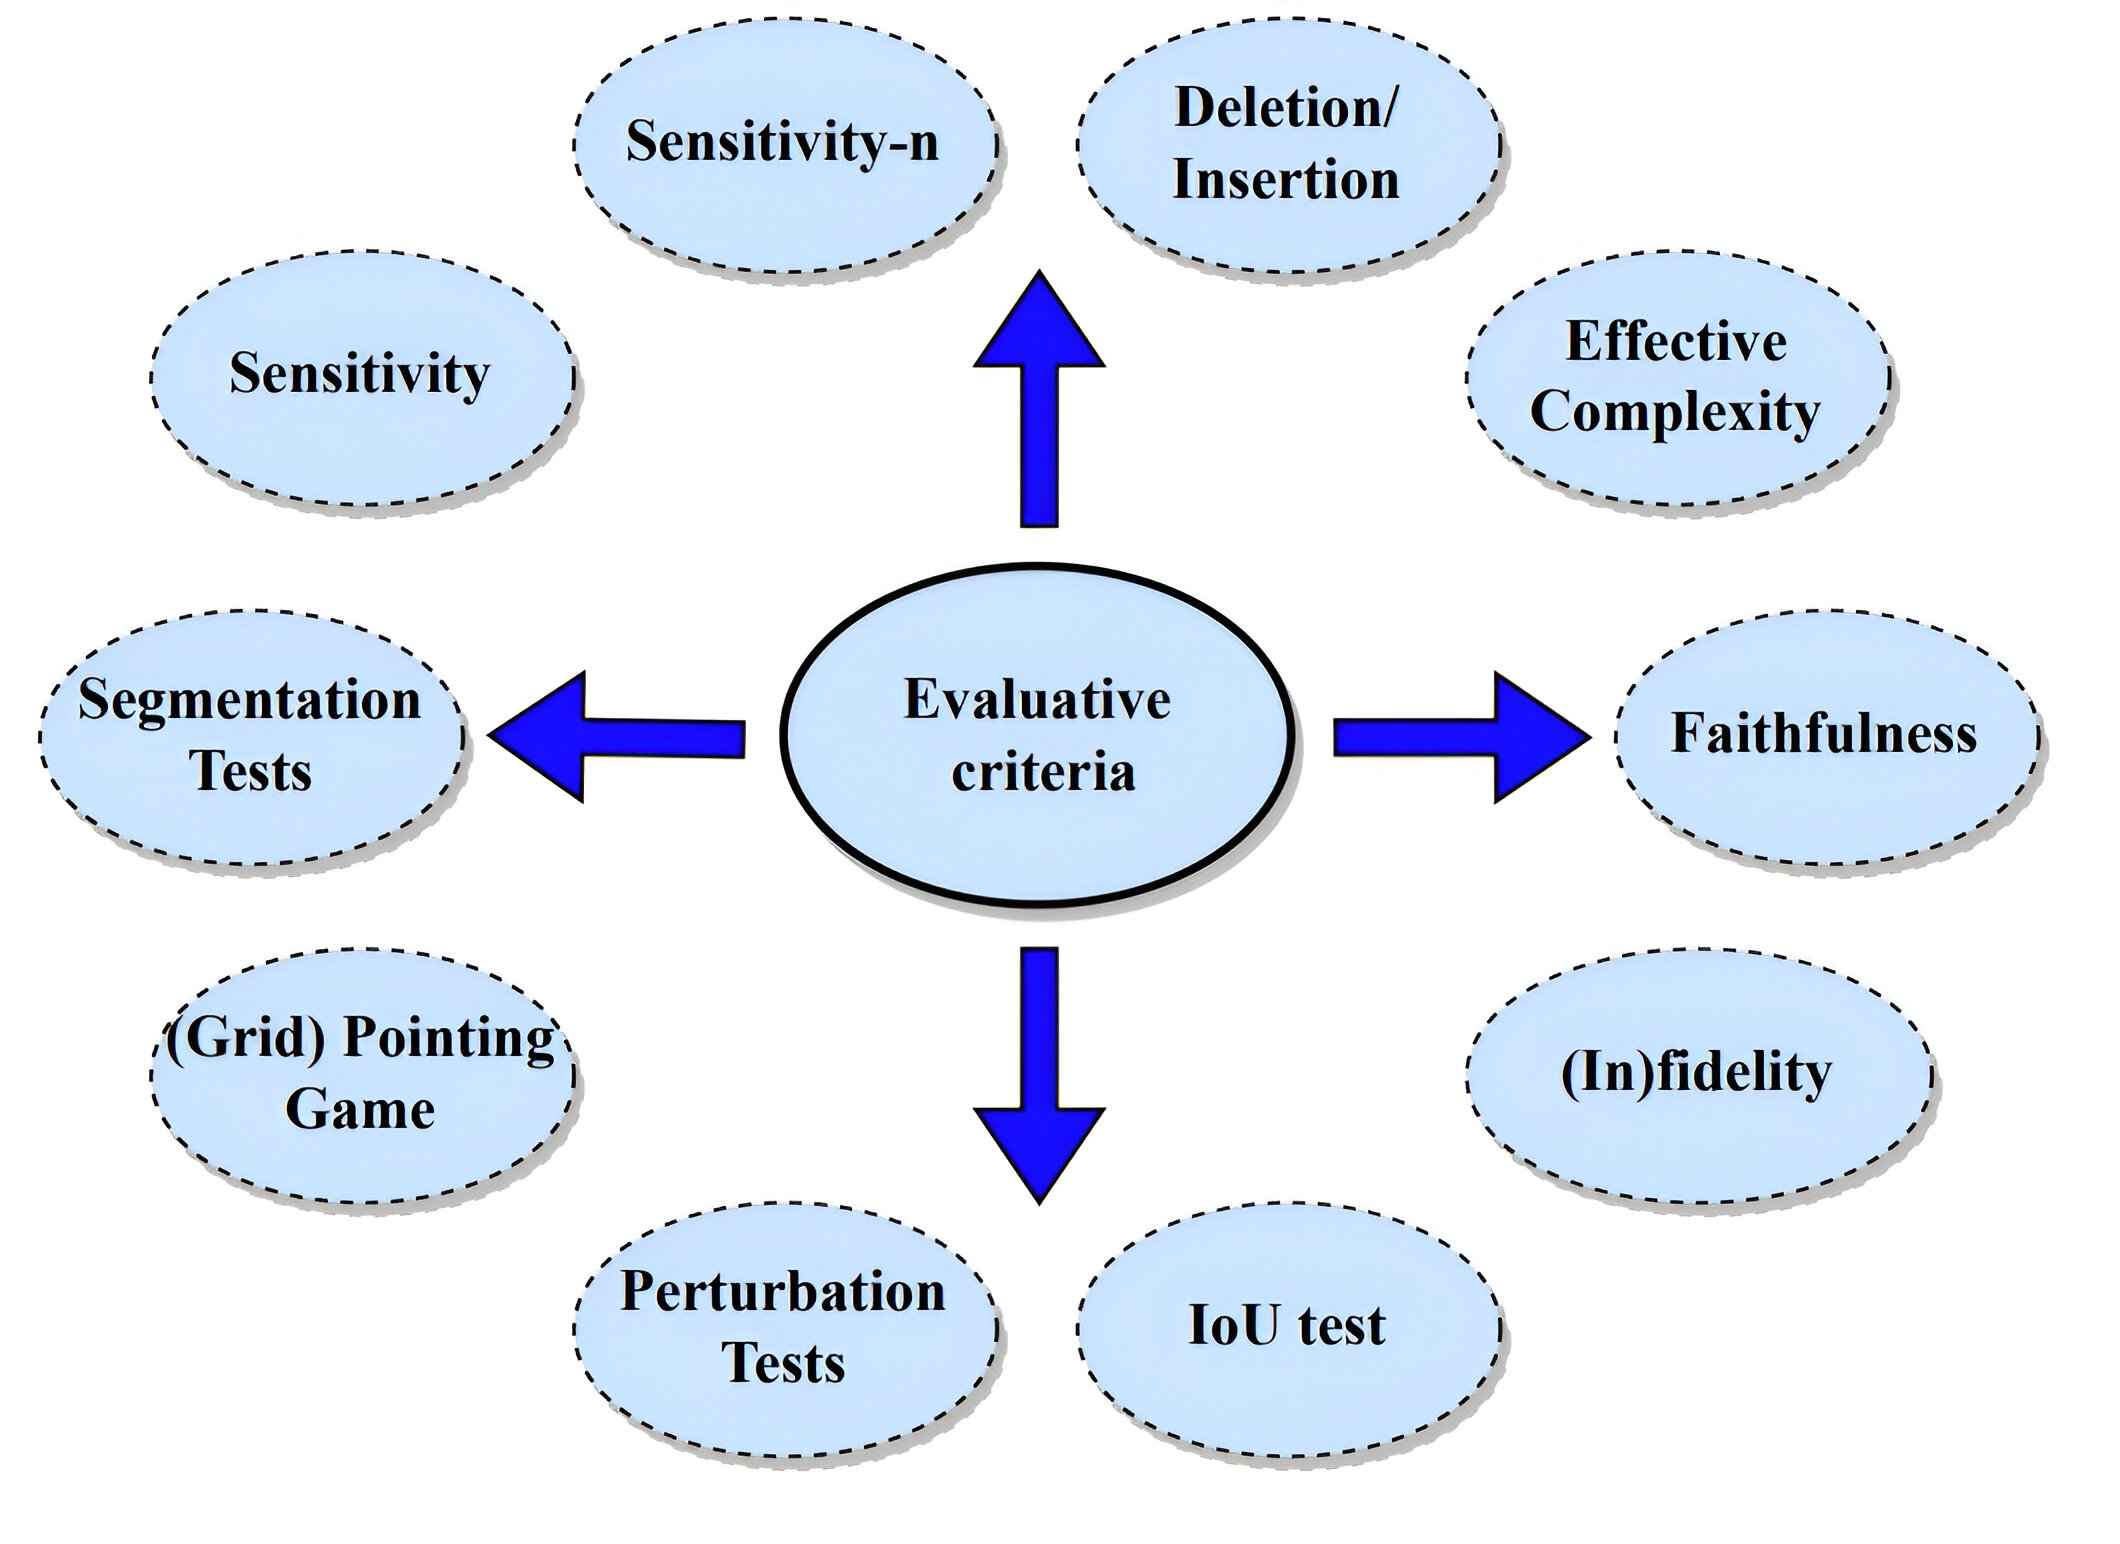
\includegraphics[width=1\textwidth]{2/figures/vt8.jpeg}
 		\caption{Diferentes criterios para evaluar los métodos de explicabilidad en aplicaciones basadas en la visiónt(\cite{tecnica1})}
 	\end{center}
 	\end{figure}
 		
 \subsubsection{Conclusión}
 
 En resumen, este trabajo ofrece una visión completa de las técnicas de explicabilidad propuestas para los transformers visuales. Hemos proporcionado una taxonomía de los métodos basada en sus motivaciones, estructuras y escenarios de aplicación, categorizándolos en cinco grupos. Además, detallamos los criterios de evaluación de la explicabilidad, así como las herramientas y marcos de trabajo utilizados. Por último, discutimos varios problemas esenciales pero poco explorados para mejorar la explicabilidad de los transformers visuales y sugerimos direcciones de investigación potenciales para futuras inversiones. Esperamos que este artículo de revisión ayude a los lectores a comprender mejor los mecanismos internos de los transformers visuales, así como a resaltar problemas abiertos para trabajos futuros.
 
 
 \subsection{You Only Look One (YOLO): You Only Look Once: Unified, Real-Time Object Detection \citep*{tecnica4}}
YOLO trata la detección de objetos como un problema de regresión, prediciendo cuadros delimitadores y probabilidades de clase directamente de imágenes completas en una sola evaluación. Esto permite una arquitectura muy rápida, procesando imágenes en tiempo real a 45 cuadros por segundo, con Fast YOLO alcanzando 155 cuadros por segundo. Aunque YOLO puede cometer más errores de localización, es menos propenso a falsos positivos de fondo y generaliza mejor a diferentes dominios como el arte.
 \subsubsection{Introducción}
En la detección de objetos, los sistemas actuales utilizan enfoques complejos que reutilizan clasificadores para detectar objetos, lo que los hace lentos y difíciles de optimizar. En contraste, el enfoque de YOLO reframes la detección como un problema de regresión única, lo que permite predecir objetos y sus ubicaciones directamente desde los píxeles de la imagen en una sola evaluación. Esto ofrece varias ventajas: en primer lugar, YOLO es extremadamente rápido, con una tasa de ejecución de hasta 150 cuadros por segundo, lo que permite el procesamiento de video en tiempo real con una latencia mínima. Además, YOLO considera globalmente la imagen al realizar predicciones, lo que le permite codificar implícitamente información contextual sobre las clases y su apariencia. Por último, YOLO aprende representaciones generalizables de objetos, lo que lo hace menos propenso a descomponerse al aplicarse en nuevos dominios o entradas inesperadas. Sin embargo, YOLO aún se queda atrás en precisión en comparación con otros sistemas de detección de vanguardia, especialmente en la localización precisa de objetos pequeños.

  \begin{figure}[H]
	\begin{center}
		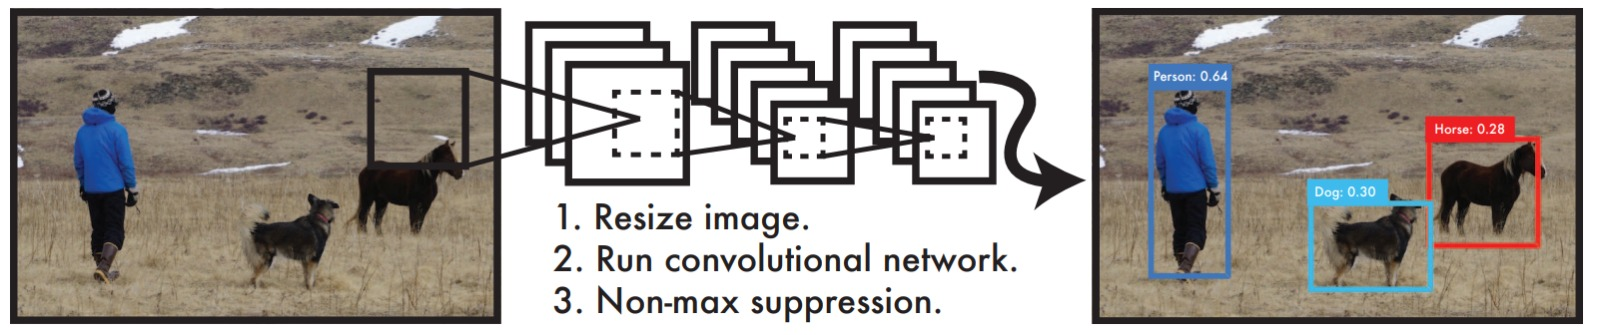
\includegraphics[width=1\textwidth]{2/figures/yolo1.jpeg}
		\caption{El sistema de detección YOLO. Procesamiento de imágenes
			con YOLO es simple y directo. Nuestro sistema (1) cambia de tamaño
			la imagen de entrada a 448 × 448, (2) ejecuta una única red convolucional en la imagen y (3) establece umbrales para las detecciones resultantes mediante
			La confianza del modelo.(\cite{tecnica4})}
	\end{center}
\end{figure}
 \subsubsection{Detección unificada}
El método fusiona todos los elementos de detección de objetos en una única red neuronal. Esta red utiliza características de toda la imagen para predecir simultáneamente las cajas delimitadoras y las clases de objetos, permitiendo un entrenamiento de extremo a extremo y velocidades en tiempo real sin perder precisión. La imagen se divide en una cuadrícula $S \times S$, donde cada celda detecta un objeto si su centro cae en ella. Cada celda predice $B$ cajas delimitadoras y sus puntuaciones de confianza, indicando la certeza del modelo sobre la presencia y precisión del objeto, además de $C$ probabilidades de clase condicionales. Durante la prueba, se combinan estas probabilidades y las predicciones de confianza para obtener puntuaciones específicas de clase para cada caja.

  \begin{figure}[H]
	\begin{center}
		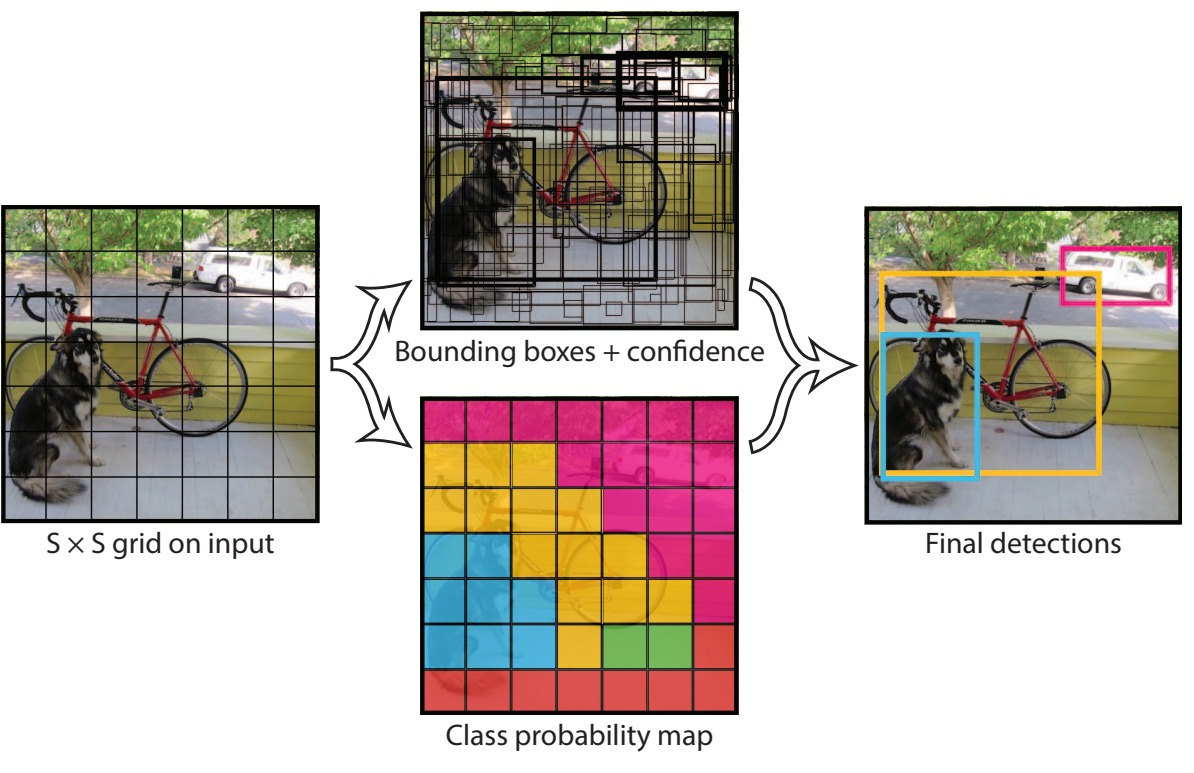
\includegraphics[width=1\textwidth]{2/figures/yolo2.jpeg}
		\caption{El sistema aborda la detección como un problema de regresión, donde la imagen se divide en una cuadrícula S × S. Para cada celda de esta cuadrícula, se predicen cuadros delimitadores, confianza asociada con esos cuadros y probabilidades de clase. Estas predicciones se codifican en un tensor con dimensiones S × S × (B x 5 + C). (\cite{tecnica4})}
	\end{center}
\end{figure}

Este modelo, una red neuronal convolucional, se evalúa en el conjunto de datos de detección PASCAL VOC. Utiliza capas convolucionales para extraer características de la imagen y capas completamente conectadas para predecir las salidas. Basado en GoogLeNet, consta de 24 capas convolucionales y 2 capas completamente conectadas. En lugar de módulos de inception, emplea capas de reducción de 1 × 1 seguidas de convoluciones de 3 × 3. Además, desarrolla una versión rápida de YOLO con menos capas convolucionales y filtros para mejorar la detección rápida de objetos.

  \begin{figure}[H]
	\begin{center}
		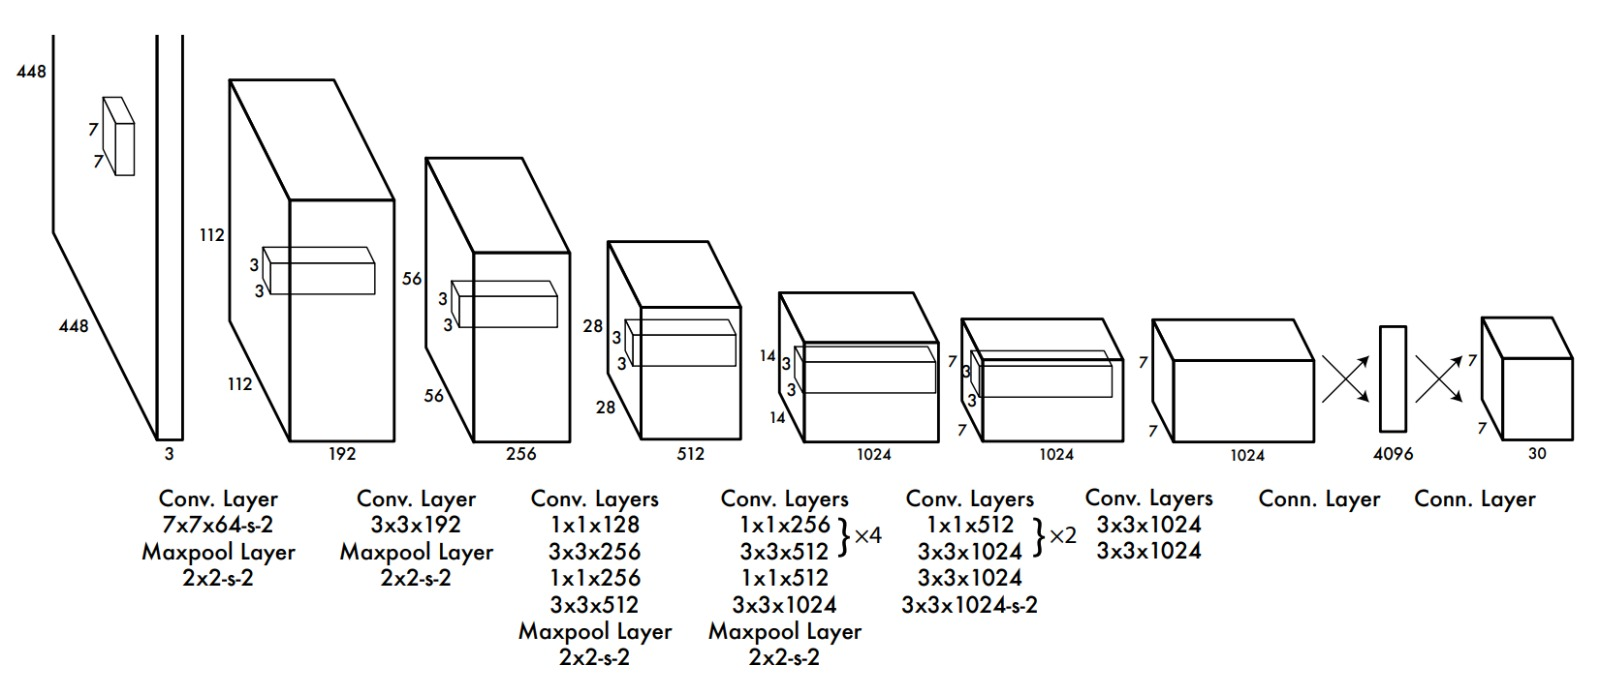
\includegraphics[width=1\textwidth]{2/figures/yolo3.jpeg}
		\caption{La red de detección consta de 24 capas convolucionales y 2 capas completamente conectadas. Se utilizan capas convolucionales de 1 × 1 para reducir el espacio de características de las capas anteriores y se preentrenan en la tarea de clasificación de ImageNet a la mitad de la resolución (224 × 224), incrementando la resolución para la detección. (\cite{tecnica4})}
	\end{center}
\end{figure}
 
\paragraph{Training} 
Las capas convolucionales se preentrenan en el conjunto de datos ImageNet de 1000 clases, logrando una precisión top-5 del 88\%. La red se convierte para la detección, aumentando la resolución de entrada de 224 × 224 a 448 × 448 para capturar detalles. La capa final predice las probabilidades de clase y las coordenadas de las cajas delimitadoras, optimizando para el error cuadrático medio. Se entrena durante aproximadamente 135 épocas en los conjuntos de datos de PASCAL VOC 2007 y 2012, utilizando un tamaño de lote de 64 y una tasa de aprendizaje variable. Durante la inferencia, predice detecciones con una sola evaluación de red, empleando supresión no máxima para corregir múltiples detecciones..

\paragraph{Limitaciones de YOLO}
YOLO impone restricciones espaciales significativas en las predicciones de las cajas delimitadoras. Cada celda de la cuadrícula solo puede predecir dos cajas y asignar una única clase, lo que limita la capacidad del modelo para detectar objetos cercanos, especialmente objetos pequeños que aparecen en grupos, como bandadas de pájaros.

Dado que el modelo aprende de los datos, enfrenta dificultades para generalizar a objetos con relaciones de aspecto nuevas o inusuales. Además, utiliza características relativamente gruesas para predecir las cajas delimitadoras debido a múltiples capas de muestreo descendente desde la imagen de entrada.

La función de pérdida utilizada durante el entrenamiento no distingue entre errores en cajas delimitadoras pequeñas y grandes, lo que puede llevar a una penalización desproporcionada por errores en cajas pequeñas, que tienen un impacto significativo en la evaluación de la superposición de IOU. En consecuencia, las localizaciones incorrectas son la principal fuente de error en nuestro modelo.

\subsubsection{Experimentos}
Se contrastó YOLO con otros sistemas de detección en tiempo real en PASCAL VOC 2007, revelando que YOLO y Fast R-CNN muestran distintos perfiles de errores. Asimismo, se evidenció la capacidad de YOLO para generalizar mejor en nuevos dominios, como conjuntos de datos de obras de arte, en comparación con otros métodos actuales en VOC 2012.

Dentro del ámbito de la detección de objetos en tiempo real, la mayoría de los esfuerzos de investigación se enfocan en mejorar la velocidad de los procesos estándar de detección. YOLO fue evaluado frente a otros métodos, resaltando su rapidez y precisión. Se introdujo una versión más ágil, Fast YOLO, que sobrepasa considerablemente a los enfoques previos en cuanto a precisión y velocidad.

Además, se examinaron otros métodos como Fastest DPM, R-CNN menos R, Fast R-CNN y Faster R-CNN, destacando sus velocidades y precisión en comparación con YOLO. Sin embargo, ninguno de ellos logra igualar el desempeño en tiempo real de YOLO.
 
 \begin{table}[H]
 	\centering
 	\caption{Comparación de Detectores en Tiempo Real y Menos que en Tiempo Real}
 	\label{tab:real-time-detectors}
 	\begin{tabular}{|l|l|l|l|}
 		\hline
 		\textbf{Detector} & \textbf{Entrenamiento} & \textbf{mAP} & \textbf{FPS} \\ \hline
 		100Hz DPM \cite{DPM} & 2007 & 16.0 & 100 \\ \hline
 		30Hz DPM \cite{DPM} & 2007 & 26.1 & 30 \\ \hline
 		Fast YOLO & 2007+2012 & 52.7 & 155 \\ \hline
 		YOLO & 2007+2012 & 63.4 & 45 \\ \hline
 		\multicolumn{4}{|c|}{\textbf{Menos que en Tiempo Real}} \\ \hline
 		Fastest DPM \cite{DPM} & 2007 & 30.4 & 15 \\ \hline
 		R-CNN Minus R \cite{RCNN} & 2007 & 53.5 & 6 \\ \hline
 		Fast R-CNN \cite{FastRCNN} & 2007+2012 & 70.0 & 0.5 \\ \hline
 		Faster R-CNN VGG-16 \cite{FasterRCNN} & 2007+2012 & 73.2 & 7 \\ \hline
 		YOLO VGG-16 & 2007+2012 & 66.4 & 21 \\ \hline
 	\end{tabular}
 \end{table}


Para examinar las diferencias entre YOLO y detectores de última generación, se realizó un análisis detallado de los resultados en VOC 2007, comparando YOLO con Fast R-CNN. Usando la metodología de Hoiem, se clasificaron las predicciones en categorías basadas en el tipo de error:

\begin{itemize}
	\item \textbf{Correcto}: clase correcta e IOU > 0.5
	\item \textbf{Localización}: clase correcta, 0.1 < IOU < 0.5
	\item \textbf{Similar}: clase similar, IOU > 0.1
	\item \textbf{Otro}: clase incorrecta, IOU > 0.1
	\item \textbf{Fondo}: IOU < 0.1 para cualquier objeto
\end{itemize}

La Figura \ref{fig:error_analysis} muestra el desglose promedio de cada tipo de error en las 20 clases. YOLO tiene más errores de localización que cualquier otra fuente combinada, mientras que Fast R-CNN comete menos errores de localización pero muchos más errores de fondo. El 13.6\% de las detecciones de Fast R-CNN son falsos positivos sin objetos, siendo casi 3 veces más propenso a predecir detecciones de fondo en comparación con YOLO.

\begin{figure}[h]
	\centering
	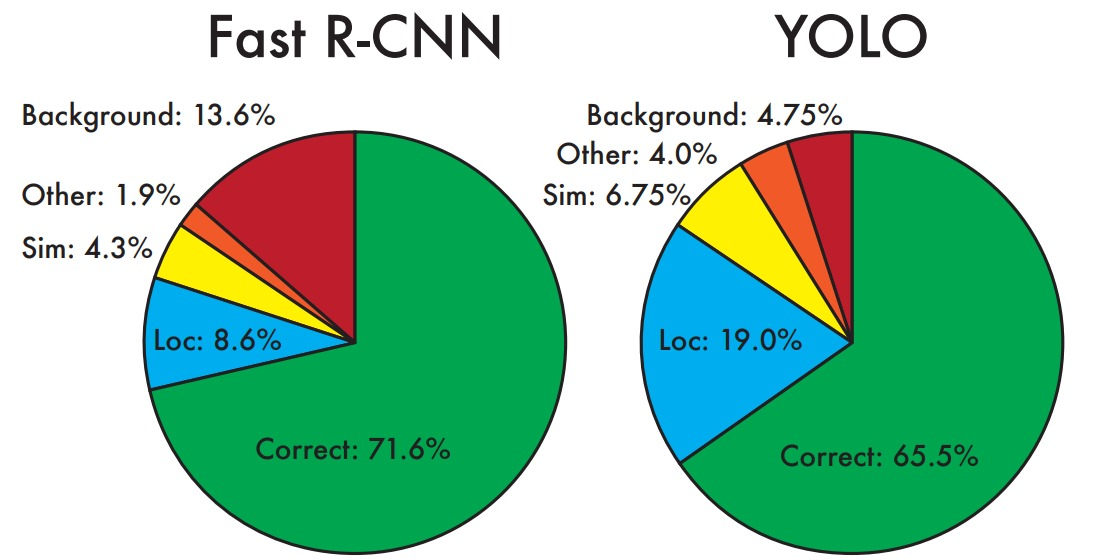
\includegraphics[width=0.8\textwidth]{2/figures/yolo4.jpeg}
	\caption{Análisis de Errores: Fast R-CNN vs. YOLO. Estos gráficos muestran el porcentaje de errores de localización y de fondo en las principales detecciones de varias categorías.}
	\label{fig:error_analysis} 
\end{figure}

YOLO comete muchos menos errores de fondo que Fast R-CNN. Al usar YOLO para eliminar las detecciones de fondo de Fast R-CNN, se obtiene una mejora significativa en el rendimiento. Por cada cuadro delimitador que predice R-CNN, se verifica si YOLO predice un cuadro similar. Si es así, se le da un impulso a esa predicción basado en la probabilidad predicha por YOLO y la superposición entre los dos cuadros.

El mejor modelo de Fast R-CNN alcanza un mAP de 71.8\% en el conjunto de prueba de VOC 2007. Cuando se combina con YOLO, su mAP aumenta a 75.0\%, con una ganancia de 3.2\%, como se muestra en la Tabla \ref{table:combination}.

\begin{table}[h]
	\centering
	\begin{tabular}{|l|c|c|c|}
		\hline
		\textbf{Modelo} & \textbf{mAP} & \textbf{Combinado} & \textbf{Ganancia} \\
		\hline
		Fast R-CNN & 71.8 & - & - \\
		Fast R-CNN (2007 data) & 66.9 & 72.4 & 0.6 \\
		Fast R-CNN (VGG-M) & 59.2 & 72.4 & 0.6 \\
		Fast R-CNN (CaffeNet) & 57.1 & 72.1 & 0.3 \\
		YOLO & 63.4 & 75.0 & 3.2 \\
		\hline
	\end{tabular}
	\caption{Experimentos de combinación de modelos en VOC 2007. Se examina el efecto de combinar varios modelos con la mejor versión de Fast R-CNN.}
	\label{table:combination}
\end{table}

El aumento de rendimiento no es simplemente un subproducto de la combinación de modelos, ya que la combinación de diferentes versiones de Fast R-CNN produce beneficios pequeños (entre 0.3 y 0.6\%). En cambio, la eficacia de YOLO se debe a que comete diferentes tipos de errores en las pruebas, lo que mejora significativamente el rendimiento de Fast R-CNN.


\subsubsection{Detección en Tiempo Real en el Mundo Real}

YOLO es un detector de objetos rápido y preciso, lo que lo hace ideal para aplicaciones de visión por computadora. Se conectó YOLO a una cámara web y se verificó que mantiene el rendimiento en tiempo real, incluyendo el tiempo para capturar imágenes desde la cámara y mostrar las detecciones.

\begin{figure}[h]
	\centering
	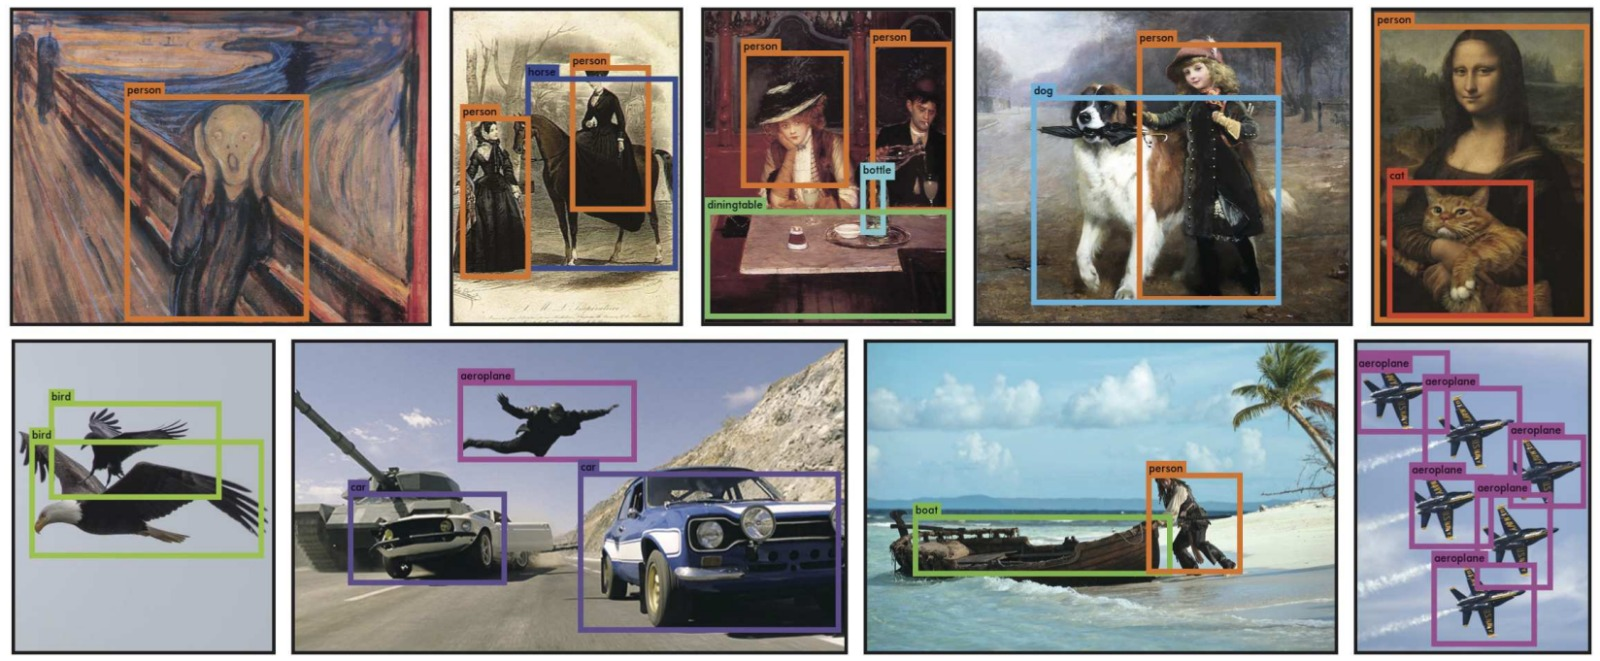
\includegraphics[width=0.8\textwidth]{2/figures/yolo5.jpeg}
	\caption{Resultados cualitativos. YOLO se ejecuta con obras de arte de muestra e imágenes naturales de Internet. Es mayoritariamente exacto, aunque cree que una persona es un avión.(\cite{tecnica4})}
	
\end{figure}

El sistema resultante es interactivo y atractivo. Aunque YOLO procesa imágenes individualmente, cuando se conecta a una cámara web funciona como un sistema de seguimiento, detectando objetos a medida que se mueven y cambian de apariencia.

\subsubsection{Conclusion}
YOLO es un detector de objetos rápido y preciso, ideal para aplicaciones de visión por computadora. Al conectarse a una cámara web, mantiene el rendimiento en tiempo real, incluyendo la captura y visualización de imágenes. El sistema es interactivo y funciona como un sistema de seguimiento, detectando objetos en movimiento

